\documentclass[12pt,a4paper]{report}

% ── Fonts ──
\usepackage{mathptmx}          % Times New Roman
\usepackage[T1]{fontenc}

% ── Page layout ──
\usepackage[margin=3cm]{geometry}
\usepackage{setspace}
\onehalfspacing
\setlength{\parskip}{6pt}
\setlength{\parindent}{0pt}

% ── Graphics ──
\usepackage{graphicx}
\graphicspath{
  {/Users/leoss/Desktop/GitHub/Capstone/FINAL CODE RECAP/Final/charts/}
  {figures/}
}
\usepackage{adjustbox}
\usepackage{float}

% ── Tables ──
\usepackage{booktabs}
\usepackage{longtable}
\usepackage{array}

% ── Math ──
\usepackage{amsmath}
\usepackage{amssymb}

% ── Hyperlinks ──
\usepackage[hidelinks]{hyperref}
\usepackage{url}

% ── Captions ──
\usepackage[font=small,labelfont=bf]{caption}

% ── Section numbering: chapter-prefix for figures and tables ──
\usepackage{chngcntr}
\counterwithin{figure}{chapter}
\counterwithin{table}{chapter}

% ── Appendix handling ──
\usepackage[toc,page]{appendix}

% ── Footnotes ──
\usepackage[bottom]{footmisc}

% ── Bibliography style ──
\usepackage{natbib}
\bibliographystyle{apalike}

% ── Suppress chapter word in headings (use just number) ──
\usepackage{titlesec}
\titleformat{\chapter}[hang]{\normalfont\LARGE\bfseries}{\thechapter}{1em}{}
\titlespacing*{\chapter}{0pt}{-20pt}{20pt}

% ── Allow deeper ToC ──
\setcounter{tocdepth}{3}
\setcounter{secnumdepth}{3}

% ══════════════════════════════════════════════════════════════
\begin{document}

% ── Title page (unnumbered) ──
\begin{titlepage}
\begin{center}
\vspace*{3cm}
{\LARGE \textbf{Beyond the Resource Curse: Industrial Upgrading\\[6pt]
In Resource-Rich Emerging Markets}}\\[2cm]
{\large LSE Capstone 2026}\\[2cm]
{\large \textbf{Candidate Numbers:}}\\[0.5cm]
{\large 59234 \quad 64689 \quad 67273 \quad 70416 \quad 73073}\\[4cm]
\vfill
\end{center}
\end{titlepage}

% ── Front matter: Roman numerals ──
\pagenumbering{roman}
\tableofcontents
\clearpage
\listoffigures
\clearpage
\listoftables
\clearpage

% ── Body: Arabic numerals ──
\pagenumbering{arabic}

% ══════════════════════════════════════════════════════════════
\chapter{Introduction}
% ══════════════════════════════════════════════════════════════

Natural resource endowments were among the earliest theoretical explanations for diverging growth trajectories between countries. Countries like China and Chile have managed to leverage their natural resources to engage in a development path. Yet these are exceptions. Across much of the developing world, rich subsoil reserves that dominate the export basket have not translated into industrial upgrading.

The failure of resource wealth to deliver sustained growth has long occupied economists. The most influential framing, the Resource Curse, holds that resource endowments can actively impede development. However, both the existence of this effect and the channels through which it operates have been subject to challenge. Since then, the literature has evolved from debating whether resources harm growth to identifying the conditions under which countries fail to convert extraction into broader productive capability. The answers point to interactions among financial depth, capital accumulation, institutional quality, and infrastructure, factors whose strong endogeneity makes isolating a single diversification narrative difficult. The sovereign risk implications, however, are clear: countries that build productive complexity develop more resilient fiscal structures, while those confined to primary extraction face persistent concentration risk in exports and revenues.

This report examines the extent to which resource-rich emerging economies diversify into higher value-added industries, using the Economic Complexity Index (ECI) to measure productive capabilities. The analysis combines a panel dataset of 54 resource-rich developing economies over 1995--2019, an econometric framework grounded in intertemporal investment theory, and machine learning models that identify relevant predictors beyond the theory-driven specification. Finally, three case studies; the Republic of Congo, Azerbaijan, and Chile; contextualise the cross-country findings.

Three pillars emerge as the most robust determinants of economic complexity: domestic credit to the private sector (financial depth), infrastructure capacity (electricity access), and human capital, both at a level and in interaction with resource intensity. Traditional macroeconomic variables contribute little predictive power once these structural determinants are accounted for. The case studies illustrate how binding constraints shift across settings: from infrastructure deficits and procyclical spending in Congo, to Dutch Disease and institutional weakness in Azerbaijan, to human capital and R\&D gaps in Chile.

The content of this report proceeds as follows. Chapter~2 reviews the resource curse literature and its mechanisms. Chapter~3 presents the quantitative analysis, including econometric results, machine learning findings, and forward projections. Chapter~4 develops three case studies. Chapter~5 concludes. Appendices provide technical and methodological detail.


% ══════════════════════════════════════════════════════════════
\chapter{Literature Review}
% ══════════════════════════════════════════════════════════════

\section{Resource Curse}

The resource curse refers to the tendency of resource-rich countries to experience lower long-run economic growth despite their natural endowments. One of the first mechanisms suggested to explain this phenomenon is that resource-rent windfalls crowd out non-resource tradeable sectors. As countries discover and export subsoil assets, their currency appreciates, rendering domestic manufacturing uncompetitive in global markets (Corden and Neary, 1982). This mechanism, known as Dutch Disease, remains central to the resource curse literature.

One of the most influential early works on the resource curse used natural resource exports as a proxy of production, instrumenting with land area (Sachs and Warner, 1995). They found that resource-intensive countries in 1971 exhibited lower growth rates between 1971--1989, relative to others. The literature further linked resource endowments to institutional deterioration, with rents incentivising rent-seeking and authoritarianism (Ross, 2015), while Collier and Hoeffler (2004) showed that commodity wealth increases the likelihood of rebellion and internal conflict. Collectively, these findings suggest resource endowments may weaken long-run growth.

In the early 2000s, Sachs and Warner (1995) faced criticism over endogeneity in its methodology, as natural resource exports themselves depend on private and public investment, institutional quality, access to electricity, and transport infrastructure. Since then, substantial research, using granular data and more rigorous methods, has found weak or no evidence for the resource curse (Poelhekke and van der Ploeg, 2010; Havr\'{a}nek, Horv\'{a}th, and Zeynalov, 2016; Lashitew, Ross, and Werker, 2020; Lederman and Maloney, 2007). This shifted the consensus toward identifying the specific conditions under which extraction leads to poor economic outcomes.


\section{Causal Mechanisms of Industrial Upgrading}

\subsection{The Logic of Industrial Upgrading}

The modern understanding of economic growth rests on the premise that development is a process of accumulating productive capabilities and deploying them into increasingly complex activities. Hausmann, Hwang, and Rodrik (2007) show that what a country exports matters, as countries producing goods in higher value-added industries tend to grow faster.

This finding is formalised in the economic complexity framework of Hidalgo and Hausmann (2009), which maps the ``product space'' and demonstrates that countries diversify by leveraging existing capabilities to move into nearby, higher-value products. Industrial upgrading is not about leapfrogging into new sectors but about incremental ``jumps'' through the product space. This is based on accumulated know-how, measured by the Economic Complexity Index (ECI), which features in our following empirical work.

The product space framework helps explain Sachs and Warner's (1995, 2001) emphasis on manufacturing, as it is the most densely connected sector and generates the strongest learning-by-doing externalities. When manufacturing contracts, a country loses not just output but the platform for future diversification. Resource-rich countries find their capabilities concentrated in extraction, far from higher-value manufactured goods in the product space. This production structure may also further reduce the learning needed to close that gap. The literature identifies several mechanisms through which this occurs.

\subsection{Institutional Quality, Expropriation, and Rent-Seeking}

A very common argument in the field is that institutional quality mediates the relationship between resource wealth and economic outcomes. Acemoglu, Johnson, and Robinson (2001, 2003) provide their theoretical foundation, showing that expropriation risk and property rights security are the fundamental determinants of long-run development. Their framework implies that resource wealth interacts with inherited institutional structures rather than through independent effects on growth.

Mehlum, Moene, and Torvik (2006) further test this hypothesis. Re-running the S\&W regressions with an interaction term between resource abundance and institutional quality, they find that resources harm growth only where institutions are ``grabber-friendly'': weak rule of law, poor contract enforcement, and high corruption. In ``producer-friendly'' institutional environments, resources are instead associated with faster growth.

This result has been influential in reframing the resource curse as conditional on governance. The mechanism operates through rent-seeking dynamics. When institutions fail to constrain elite capture, resource rents are diverted from productive investment into patronage, consumption, and political consolidation. Acemoglu et al.\ (2019) further demonstrate that democratic institutions, which impose stronger constraints on rent extraction, are causally associated with higher long-run GDP.

\subsection{Human Capital and Savings Rates}

Resource dependence may also limit industrial upgrading through its effects on human capital accumulation and savings behaviour. Gylfason (2001) provides cross-country evidence that natural resource abundance is negatively associated with public education expenditure, school enrolment, and expected years of schooling. Resource booms raise the opportunity cost of education by offering high wages in extraction for unskilled labour, while governments with increased fiscal capacity face reduced incentives to invest in human capital, since their fiscal base does not depend on a skilled workforce.

These patterns reflect a deeper political economy problem. In resource-rich states, the social contract between taxation and public service provision is weakened because revenues derive primarily from extraction rather than from taxing a productive citizenry (Van der Ploeg and Venables, 2011). This generates underinvestment and decreases diversification incentives, even when formal institutional quality is not the binding constraint.

\subsection{Price Volatility, Credit Ratings, and Investment}

Primary commodity prices are inherently volatile, and this volatility transmits directly into the fiscal revenues, exchange rates, and growth trajectories of dependent economies. As such, they have gained prominence as a mechanism through which heavy primary resource dependence becomes costly.

Van der Ploeg and Poelhekke (2009) show that resource abundance boosts growth directly but undermines it through volatility, consistent with the conditional curse framework: resources are not inherently harmful, but their macroeconomic side effects concentrate in countries lacking the institutional and financial capacity to manage them. Under credit constraints, volatility shifts investment composition away from long-term, high-return projects toward short-term, low-return alternatives (Aghion, Angeletos, Banerjee, and Manova, 2010).

These dynamics feed into sovereign creditworthiness. Mlachila and Ouedraogo (2020) find that commodity price shocks drive financial underdevelopment in resource-rich countries, mitigated only by strong governance. Manzano and Rigobon (2001) go further, arguing that the apparent resource curse might be a debt overhang problem: countries borrowed against future resource revenues during the 1970s commodity boom, and the resulting debt burden explains their subsequent poor growth. This interpretation reinforces the conditional view that the issue lies in the financial choices made because of resource abundance, rather than resource abundance itself.

\subsection{Point-Source Resources as an Exacerbating Factor}

Not all natural resources carry the same developmental risks. The literature distinguishes between geographically concentrated, capital-intensive commodities (``point-source'') and more dispersed ones, produced by a broader base of economic actors (``diffused''). Isham et al.\ (2005) posit that point-source exports are associated with weaker institutional outcomes. This is because they generate larger, more concentrated rents, that are easier for narrow elites to appropriate and harder for broad-based coalitions to monitor. Boschini et al.\ (2007) show that the interaction between resource type and institutional quality is decisive: appropriable resources such as oil and diamonds are significantly more damaging in weak institutional settings but can be managed productively where institutions are strong.

These findings raise the question of where forestry sits within this typology. Conventionally grouped with agriculture as a diffuse, renewable resource, industrial forestry in many developing countries governs more like mining: tropical forests are overwhelmingly state-owned, with extraction rights allocated through concession contracts that mirror mineral concessions (Piketty et al., 2008; FAO and EFI, 2018). Corruption in these contracts parallels patterns in the mining sector, depriving governments of significant revenues through opaque allocation and regulatory capture (S{\o}reide, 2007).

Despite these similarities, Bhattacharyya and Collier (2014) show that rents from non-renewable mineral depletion reduce the public capital stock, while rents from forestry and agriculture do not. Thus, forestry occupies an intermediate position between the point-source and diffuse categories.

\subsection{Summary}

The literature identifies several interacting mechanisms through which natural resource dependence may impede industrial upgrading: Dutch Disease effects on manufacturing competitiveness, institutional deterioration through rent-seeking, underinvestment in human capital, macroeconomic volatility from commodity price swings, and the particular risks associated with point-source resources. However, none of these mechanisms operates deterministically. The empirical evidence increasingly points to conditional effects, where institutional quality, savings behaviour, and the type of resource extracted mediate the relationship between endowments and development outcomes.


% ══════════════════════════════════════════════════════════════
\chapter{Quantitative Analysis}
% ══════════════════════════════════════════════════════════════

The literature review establishes two broad findings. First, the negative causal relationship between resource abundance and economic growth lacks consistent empirical support. Second, that resource-rich countries' development outcomes depend on interacting factors including institutional quality, human capital, fiscal management, infrastructure, and resource type.

Our objective now is to assess the ability of resource-rich countries to upgrade their value chain, the process by which economies move from exporting commodities to more knowledge-intensive activities. To do this, we employ the Economic Complexity Index (ECI) as the outcome of interest, which measures the diversity and sophistication of a country's export basket (see Appendix~A). A country with a rising ECI is accumulating the capabilities needed to move into higher-value activities; a country with a declining ECI is losing them. Our quantitative models evaluate the relative importance of the factors identified in the literature and their relationships with natural resource production.

To conduct the quantitative analysis two complementary empirical approaches are employed. The \textbf{econometric framework} uses panel regressions to test a specific hypothesis drawn from the theoretical discussion: that human capital and physical capital accumulation interact with the intensity of resource production to predict changes in economic complexity. This specification, based on the intertemporal investment argument of Venables (2016), allows us to estimate interpretable coefficients and compare our results directly with prior work. The \textbf{machine learning (ML) framework} takes a more agnostic approach. By including a broader set of variables and allowing the data to determine which predictors matter most, the ML analysis can detect patterns that the theory-driven econometric model may miss, while also serving as a cross-validation of the econometric findings.


\section{Data}

We construct a country-level panel dataset covering the period 1995--2019. This incorporates variables across a broad set of dimensions that may influence an economy's capacity to move into more complex and higher value-added activities. The dataset includes: (i) natural resource endowment indicators, covering both resource rents and production volumes; (ii) macroeconomic variables; (iii) fiscal and financial indicators; (iv) governance measures; (v) indicators capturing the GDP structure of each country; (vi) human capital variables; (vii) infrastructure indicators; and (viii) geographical and other structural characteristics.

The variable choices and their sources are summarised in Table~\ref{tab:data_vars} and Figure~\ref{fig:data_sources}. Most of the data draws from the World Bank World Development Indicators, which supplies most macroeconomic, structural, financial and human capital variables. Governance indicators are sourced from the Varieties of Democracy (V-Dem) dataset. Factor inputs and productivity measures come from the Penn World Tables version 11.0 (PWT 11.0). Macroeconomic flow variables, including government finance aggregates, are supplemented from the International Monetary Fund (IMF). Natural resource production data are drawn from the Energy Institute and Our World in Data (EI/OWID). Additional details on each variable and its source are provided in Appendix~A.

\begin{figure}[H]
\centering
\adjustbox{max width=\linewidth}{\includegraphics{image2}}
\caption{Data variables}
\label{tab:data_vars}
\end{figure}

\begin{figure}[H]
\centering
\includegraphics[width=0.95\textwidth]{image3}
\caption{Data sources by macro-indicator}
\label{fig:data_sources}
\end{figure}

\subsection{Country Selection}

To avoid arbitrarily selecting our countries of interest, we conduct our analysis on developing countries where natural resource rents exceeded 5\% of GDP in 1995. This threshold is intended to ensure that natural resources represent a structurally significant component of economic activity rather than a marginal income source. Countries classified as high-income by the World Bank in 1995 are excluded, restricting the sample to developing and middle-income economies. A special treatment is made for Gulf states, as their 1995 income class does not reflect the level of industrial upgrading. Therefore, despite being classified as high-income in 1995, these countries are retained in our sample. Several countries that would otherwise satisfy these criteria are excluded on data availability grounds. The complete list and the rationale for each exclusion are provided in Appendix~B. The final sample comprises 54 countries, shown in Figure~\ref{fig:sample_map}.

Any remaining gaps are filled by linear interpolation within each country's time series, with extrapolation capped at three years beyond the nearest observed value to avoid projecting short-run patterns over long horizons (Appendix~B). Where a country has no observed value for a variable across the entire sample period, a second pass uses K-Nearest Neighbours (KNN, $k = 5$, distance-weighted) to fill the missing cell from the five most similar country-year observations (Appendix~B).

\begin{figure}[H]
\centering
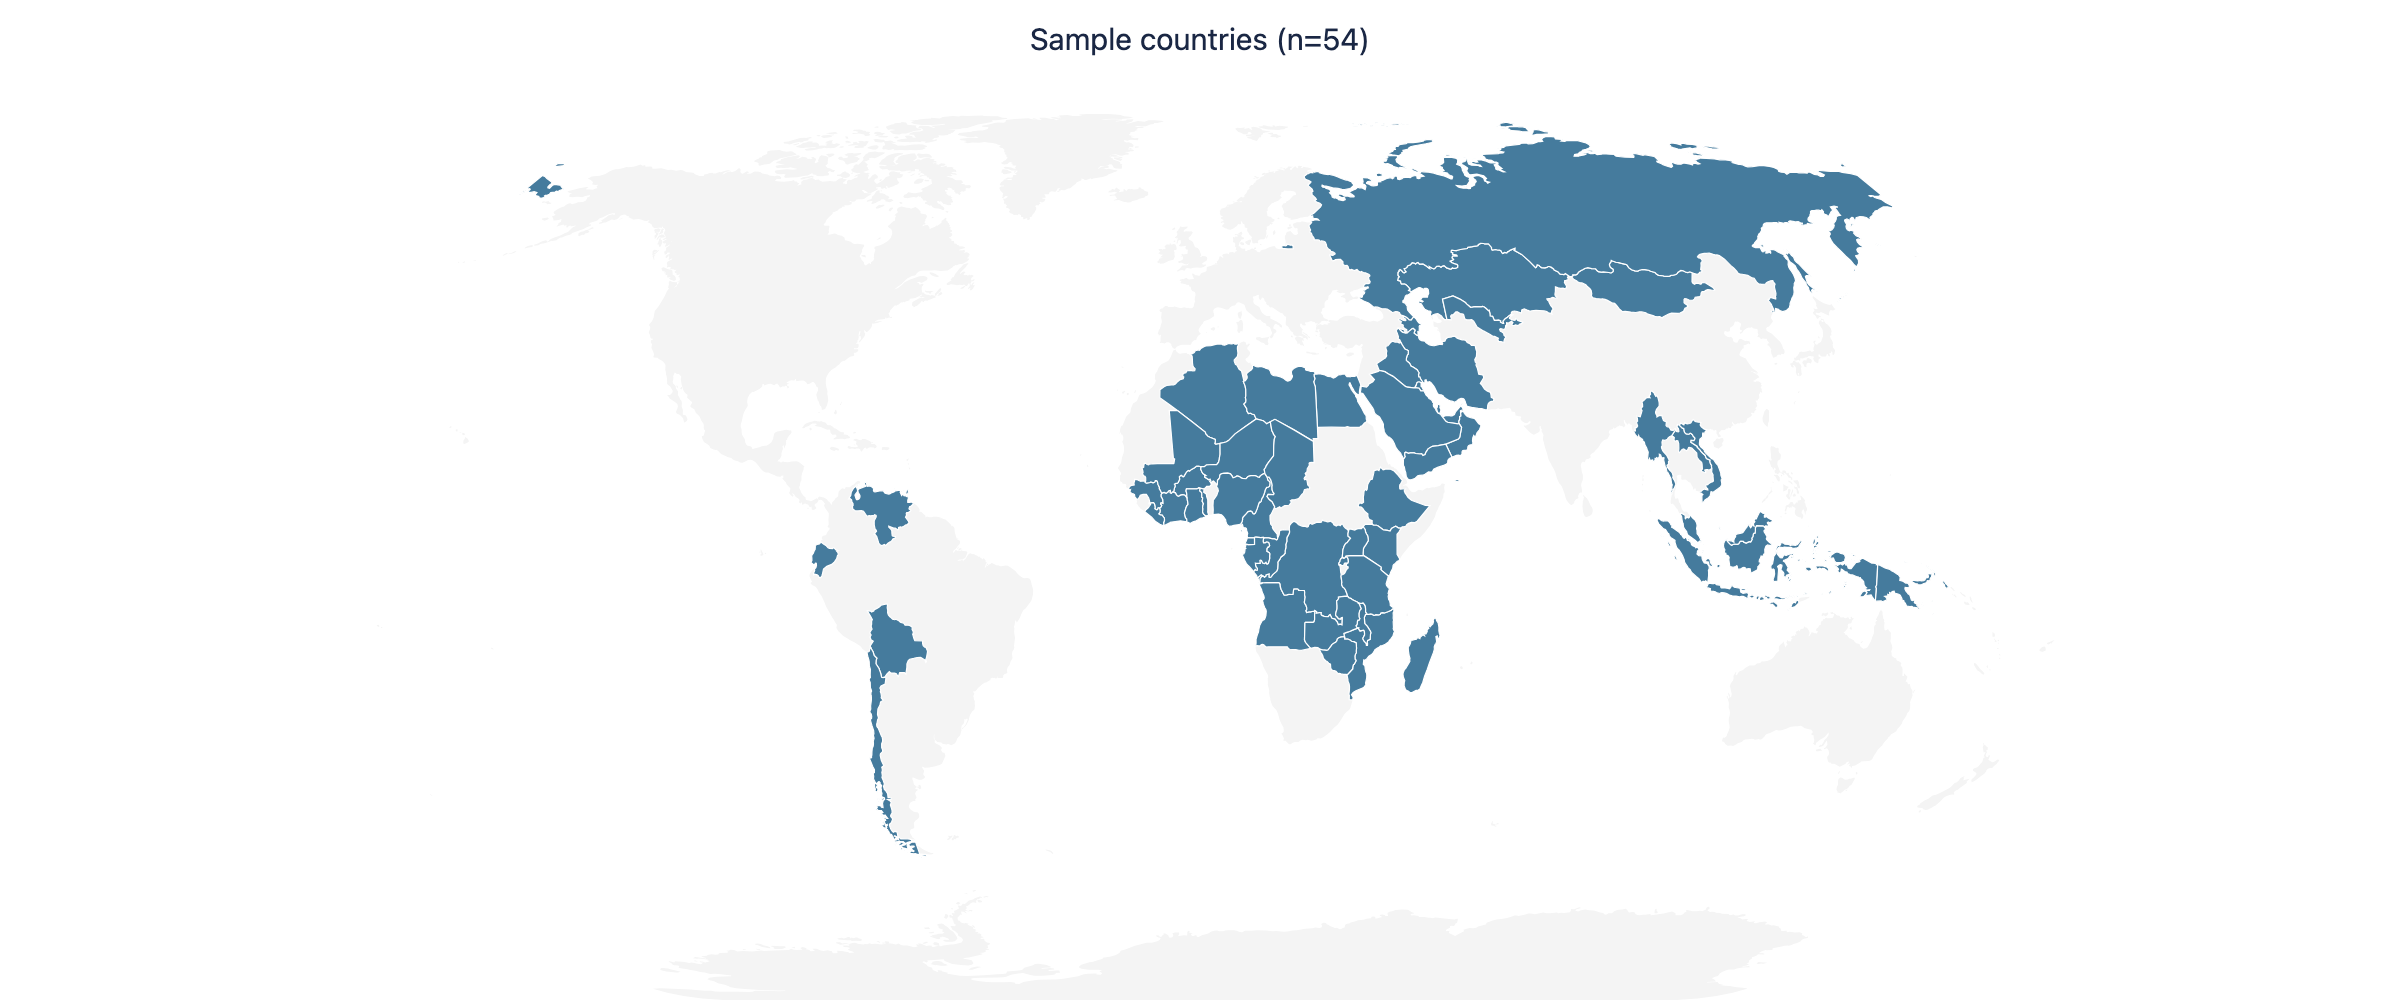
\includegraphics[width=0.95\textwidth]{descriptive/chart000_sample_map}
\caption{Countries in the sample}
\label{fig:sample_map}
\end{figure}


\section{Descriptive Statistics of the Sample}

The high-resource subsample shows a lower mean ECI ($-0.760$ versus $-0.070$), consistent with resource-rich economies having a generally lower level of productive diversification. Human capital, proxied here by the Human Capital Index (HCI), is also modestly lower in the high-resource subsample, while natural resource production value per capita is, by construction, substantially higher.

These patterns reflect well-documented features of resource-dependent economies. Productive diversification into more complex goods requires functioning credit markets, a skilled workforce, and the institutional conditions that correlate with lower corruption and longer life expectancy. Table~\ref{tab:desc_stats} presents descriptive statistics for the full sample of 3,150 country-year observations and for the restricted subsample of high-resource countries (1,350 observations). Figure~\ref{fig:correlations} shows Pearson correlations between ECI and the candidate variables. The strongest positive associations are with domestic credit, the human capital index, and life expectancy. The strongest negative are with political corruption and agricultural value added as a share of GDP, the latter reflecting the standard structural shift away from primary activity as complexity rises. These correlations motivate the variable selection in the regression and machine learning stages that follow.

\begin{figure}[H]
\centering
\adjustbox{max width=\linewidth}{\includegraphics{image5}}
\caption{Descriptive statistics}
\label{tab:desc_stats}
\end{figure}

\begin{figure}[H]
\centering

\includegraphics[width=0.95\textwidth]{descriptive/02_correlations_with_eci}
\caption{Correlation of features with ECI}
\label{fig:correlations}
\end{figure}


\section{Clustering Countries by Natural Resource Production}

As an exploratory exercise, we conduct clustering, a technique that identifies groups of similar observations based on their characteristics. In our case, we cluster based on the resource profile of each country, grouping them in different sections. This helps us understand the different types of resource intensiveness.

The clustering proceeds in two stages. First, we apply Principal Component Analysis (PCA), which compresses many correlated resource variables into just two, while still capturing most of the variation in the data. Second, we apply K-means clustering to these summary dimensions, where each country is assigned to a group based on how similar it is to other ones. A more in-depth explanation of the clustering process is included in Appendix~C.

\subsection{Principal Component Analysis}

PCA transforms the production values for each resource of interest into a smaller set of variables. These are called principal components (PCs), each constructed to capture as much of the remaining variance in the data as possible. Compressing multiple indicators into just a few discards some information about the sample, but by maximising the variance retained at each step, PCA limits this loss while improving interpretability.

We carry out this technique for two reasons. First, rather than preselecting which resources to cluster on, the approach allows the data itself to reveal which minerals and hydrocarbons account for the most cross-country variation. Second, it provides a less noisy set of inputs to the K-means algorithm, which tends to improve both clustering stability and interpretability.

We retain the first two principal components, which together account for 70\% of total variance in the standardised data. Around 30\% of the information available in the sample is lost, but this is an acceptable trade-off given the reduction from 21 resource variables to just two composite dimensions. PC1 captures the largest share of variance and loads most heavily on oil and natural gas, effectively separating hydrocarbon producers from the rest of the sample. PC2 is driven by copper, gold, and coal, distinguishing countries whose extraction is concentrated in mining. The full set of factor loadings and variance shares are reported in Figure~\ref{fig:pca_biplot} and discussed in Appendix~C.

\subsection{K-means Clusters}

To group countries with similar extraction profiles, we apply K-means clustering to the country value on the first two principal components. K-means partitions observations into a pre-specified number of groups by minimising the distance (extraction profiles) between members of the same group (or cluster). We set the number of clusters to five and use production data for 1995; Appendix~C discusses alternative choices regarding the number of clusters, the year selected, and the variables included. The resulting groupings are described below:

\begin{enumerate}
\item \textbf{Petrostates} comprises countries with very high oil or gas endowments and limited mineral production. Saudi Arabia, Kuwait, the UAE, Qatar, Oman, and Bahrain all mainly rely on hydrocarbons and tend to have very high production figures per capita.

\item \textbf{Oil Exporters} captures countries with moderate oil or gas output alongside limited mineral activity. Unlike the petrostate group, these economies are less dominated by a single commodity and tend to have lower per-capita hydrocarbon revenues. The cluster includes Ecuador, Angola, Nigeria, Egypt, Iraq, Libya, Algeria, Republic of the Congo, Azerbaijan, Trinidad and Tobago, and Gabon.

\item \textbf{Major Producers} groups countries with significant and often diversified production spanning both hydrocarbons and minerals. Russia, Kazakhstan, Indonesia, Papua New Guinea, Uzbekistan, Bolivia, and Malaysia occupy a wide range of extraction profiles.

\item \textbf{Mining Exporters} contains Chile and Mongolia, which produce mainly minerals rather than hydrocarbons.

\item \textbf{Forestry Intensive} includes countries with smaller-scale or less diversified extractive sectors, such as the Democratic Republic of Congo, Zimbabwe, Ghana, Guinea, Mali, Niger, and Vietnam. Many of these countries entered the sample primarily through forestry rents rather than mineral or hydrocarbon extraction.
\end{enumerate}

Figures~\ref{fig:pca_biplot} and~\ref{fig:cluster_map} confirm that these five groups occupy distinct regions of the resource space. In the PCA biplot (Figure~\ref{fig:pca_biplot}), Petrostates and Oil Exporters are pulled toward the right by oil and gas loadings, Mining Exporters sit high on the copper and gold axis, and Forestry Intensive countries cluster in the lower-left corner with weak loadings on all major resources. The clusters are not regionally determined, as they often span continents (Figure~\ref{fig:cluster_map}). Countries outlined in black in Figure~\ref{fig:cluster_map} are major global producers, contributing over 15\% of world output for at least one resource.

\begin{figure}[H]
\centering
\includegraphics[width=0.95\textwidth]{image7}
\caption{K-means clusters in PCA space ($K=5$)}
\label{fig:pca_biplot}
\end{figure}

\begin{figure}[H]
\centering

\includegraphics[width=0.95\textwidth]{descriptive/04_cluster_world_map_k5}
\caption{Natural resource clusters mapped by country (1995)}
\label{fig:cluster_map}
\parbox{0.9\textwidth}{\small\textit{Note: Black border indicates major global producer ($>$15\% of a resource's world production).}}
\end{figure}

Understanding how these groups differ in ECI helps identify how each resource type correlates with development. Figure~\ref{fig:eci_trajectory} plots the median ECI for each cluster between 1995 and 2019. Petrostates remain the most complex economies in the sample, while Oil Exporters consistently record the lowest median complexity. Resource type alone does not explain these gaps: the two hydrocarbon-based clusters end up at opposite ends of the complexity distribution. Oil Exporters record median ECI levels around 0.2 to 0.3 points below Forestry Intensive economies throughout the panel (Figure~\ref{fig:eci_trajectory}), despite recording the highest normalised oil rents in the sample (Figure~\ref{fig:cluster_profiles}). This aligns with the point-source versus diffuse resource distinction: hydrocarbon rents are easier for narrow elites to capture, while forestry operates through a broader economic base. Diversified Producers and Mining Exporters converge near the middle of the distribution by 2019.

Figure~\ref{fig:cluster_profiles} completes the picture. Petrostates approach Mining Exporters in GDP per capita, while Oil Exporters and Forestry Intensive countries rank lowest on income, credit access, and human capital. Mining Exporters, driven largely by Chile, record the strongest governance and human capital scores. Governance quality, human capital, and credit access vary widely even within similar resource bases, suggesting these characteristics matter more for complexity than the commodities extracted. The econometric and machine learning analyses that follow test this formally.

\begin{figure}[H]
\centering

\includegraphics[width=0.95\textwidth]{descriptive/15_eci_trajectory_by_cluster_k5}
\caption{Evolution of Economic Complexity vs.\ log GDP per capita (PPP), 1995--2019}
\label{fig:eci_trajectory}
\end{figure}

\begin{figure}[H]
\centering

\includegraphics[width=0.95\textwidth]{descriptive/06_cluster_profile_comparison_k5}
\caption{Difference between clusters}
\label{fig:cluster_profiles}
\end{figure}


\section{Econometrics Approach}

\subsection{Background}

The econometric analysis tests a conditional resource explanatory mechanism. While most empirical research has focused on institutional quality as the primary mediating factor (Acemoglu, Johnson, and Robinson, 2001; Mehlum, Moene, and Torvik, 2006), the role of how resource revenues are saved and invested has received less attention. Therefore, we rely on Venables (2016) intertemporal allocation framework, where resource-rich countries choose between consuming extraction revenues or converting them into physical infrastructure, human capital, and financial assets that sustain income post-depletion. While poorer countries may save less given higher marginal utility of consumption, Venables argues that observed savings rates in resource-rich economies remain below optimal levels, constraining structural transformation.

We test this argument empirically by testing whether capital accumulation, both physical and human, is associated with higher economic complexity, and whether this association is stronger in countries with more intensive resource production. If the framework is correct, the investment returns are greater where resource production is large, because in those settings the gap between current and optimal capital stocks is widest and the potential gains from investment greatest.

We also test for differentiated impacts from subsoil versus forest assets. Given that subsoil resources (oil, gas, coal, minerals) are more geographically concentrated, point-source commodities would make this effect more pronounced, yielding larger investment returns than for forest assets.

\subsection{Model}

Estimating the impact of capital accumulation on economic complexity in resource-dependent countries is challenging due to endogeneity. Discovering and extracting resources require a productive capability baseline. However, causation among institutions, investment, and extraction is difficult to establish. Good institutions may give rise to the firms and coordination needed to operate mining activities, or alternatively, income from extraction may fund the institutional development that producers demand to protect their returns. Similar arguments apply to trade openness, credit access and infrastructure: each plausibly causes and is caused by the level of economic complexity. We cannot fully resolve these issues and are unable to infer causality through this analysis.

The Human Capital Index (HCI) and Gross Fixed Capital Formation as a share of GDP (GFCF) serve as measures of human and physical capital accumulation respectively. We use production to capture natural resource intensity measured as the total value of natural resource assets produced each year and calculated as physical output quantities multiplied by world prices and divided by population. To capture output from forestry extraction, we include Forestry Rents as a percentage of GDP. Political stability, rule of law, and trade openness enter as controls for the institutional and conditions emphasised in broader literature.

We are also including interaction terms to test for non-linearities: \textit{HCI $\times$ Production} and \textit{GFCF $\times$ Production}, \textit{HCI $\times$ Forestry Rents}, and \textit{GFCF $\times$ Forestry Rents}. A positive coefficient on either would indicate that capital accumulation is associated with larger gains in economic complexity at higher levels of resource production, consistent with the hypothesis that the returns to converting resource wealth into productive capital are greatest where extraction is most intensive. Interaction terms are computed on mean-centred logged variables.

Our identification strategy relies on country-clustered standard errors. Standard OLS assumes independent and identically distributed errors; however, in panel data, observations from the same country across years are likely correlated. Ignoring this would produce artificially small standard errors and inflated $t$-statistics, leading to spurious significance. Ideally, we would also include country fixed effects to address omitted variable bias from time-invariant, country-specific characteristics. However, the limited number of country clusters in our sample makes it infeasible to implement both simultaneously. Faced with this trade-off, we prioritised accurate inference through clustering over correcting for potential coefficient bias through fixed effects. Therefore, results should be interpreted with the caveat that coefficient estimates may be biased by unobservable, time-invariant country characteristics.

Because ECI is highly path-dependent, a country's productive capabilities in one year are strongly correlated with its capabilities the following year. As a result, the regression includes a one-period lag of ECI. As a robustness check for reverse causality, we re-ran the regression using all lagged variables. The following equations describe Models~(1) and~(2):

\begin{equation}
\begin{split}
ECI_{it} = \beta_0 + \beta_1 HCI_{it} + \beta_2 GFCF_{it} + \beta_3 Production_{it} + \beta_4 PoliticalStability_{it} \\
+ \beta_5 RuleOfLaw_{it} + \beta_6 Trade_{it} + \beta_7 ForestryRents_{it} \\
+ \beta_8 HCI_{it} \times Production_{it} + \beta_9 GFCF_{it} \times Production_{it} \\
+ \beta_{10} HCI_{it} \times ForestryRents_{it} + \beta_{11} GFCF_{it} \times ForestryRents_{it} + \epsilon_{it}
\end{split}
\end{equation}

\begin{equation}
\begin{split}
ECI_{it} = \beta_0 + \beta_1 HCI_{it} + \beta_2 GFCF_{it} + \beta_3 Production_{it} + \beta_4 PoliticalStability_{it} \\
+ \beta_5 RuleOfLaw_{it} + \beta_6 Trade_{it} + \beta_7 ForestryRents_{it} \\
+ \beta_8 HCI_{it} \times Production_{it} + \beta_9 GFCF_{it} \times Production_{it} \\
+ \beta_{10} HCI_{it} \times ForestryRents_{it} + \beta_{11} GFCF_{it} \times ForestryRents_{it} \\
+ \beta_{12} ECI_{i,t-1} + \epsilon_{it}
\end{split}
\end{equation}

\subsection{Results}

Table~\ref{tab:regression} reports the estimates across the three specifications. The Human Capital Index enters positively and significantly in every model, showing the effect is robust. The coefficient falls once lagged ECI is introduced (from 1.643 in Model~1 to 0.286 in Model~2 and 0.278 in Model~3) because much of the cross-country variation in human capital is absorbed by the lagged term, which captures the accumulated stock of productive capabilities. HCI remaining significant even after adding this variable indicates that human capital accumulation contributes to complexity growth beyond what is already embedded in a country's existing trajectory. Lagged HCI is significant, showing that previous levels of Human Capital increase ECI in the following period. Gross Fixed Capital Formation follows a similar pattern, entering positively and significantly across all specifications.

Production Value, our measure of resource extraction intensity, is negative throughout all models but none of the coefficients is significant. The direction is consistent with the literature: among resource-rich countries, higher per-capita extraction is associated with lower complexity, though the lack of significance suggests this direct effect is negligible once other variable effects are accounted for. Forestry Rents follows a similar pattern.

None of the four interaction terms is significant across the three specifications. However, three of the four interaction terms are positive across all specifications. A positive coefficient suggests that the association between human capital/gross fixed capital and economic complexity is stronger in countries with more intensive resource production, consistent with Venables (2016) argument that human capital investment yields larger returns precisely where the gap between existing capabilities and the requirement for diversification is widest. The results suggest that the composition of human capital and physical investment matters more at the aggregate level regardless of the resource dependence.

Among the controls, institutional variables (political stability, rule of law, trade openness) are not individually significant in Models~(2) and~(3), likely because within-country variation between 1995--2019 is insufficient to generate a detectable signal once accounting for ECI trajectory. The lagged dependent variable dominates the explained variance in Models~(2) and~(3), with $R^2$ rising from 0.371 in Model~1 to 0.787 in Models~2 and~3. The all-lagged specification, which lags all regressors by one period to address simultaneity, produces closely consistent results; HCI and GFCF remain significant at comparable levels, while natural resource production variables and all the interaction terms remain non-significant.

We also estimated a model with the change in ECI as the dependent variable as a robustness check. Results are reported in Appendix~D. Despite a notable decrease in $R^2$, from 0.789 to 0.095, the coefficients and standard errors of the variables of interest remain stable in sign, magnitude, and significance.

\begin{figure}[H]
\centering
\adjustbox{max width=\linewidth}{\includegraphics{image11}}
\caption{Regression results}
\label{tab:regression}
\end{figure}


\section{Machine Learning Approach}

The econometric framework is developed reviewing economic theory and research on the role natural resources play in economic development. The choice of predictors is therefore decided before the model is estimated. This guards against p-hacking (the practice of testing many specifications until a significant result appears) and ensures interpretable coefficients. At the same time, variables which matter empirically, but lack a clear theoretical motivation, may be excluded. As a result, the model becomes susceptible to misspecification of functional form and omitted variable bias (Belloni et al., 2014).

We therefore complement the econometric analysis by using Machine Learning (ML) techniques. Our models of choice (LASSO, Ridge, Elastic Net, and Random Forest) take a more agnostic approach to variable selection. These models are able to test the predictive power of a broad set of candidate predictors, testing their relationship with economic complexity, as well as their reliability when applied to new data. To avoid reliance on outliers or spurious relationships, we utilise regularization methods (LASSO, Ridge, Elastic Net) that shrink or eliminate coefficients associated with weak predictors, and ensemble methods like Random Forest, that average the predictions of many individual decision trees to reduce instability. Together, these tools serve as a check on the econometric findings.

\subsection{Regularisation Techniques}

All regularisation techniques discussed here share the same linear modeling framework as Ordinary Least Squares (OLS). They assume a linear relationship between the dependent variable and the predictors, estimate coefficients by minimising deviation from the fitted curve and test how much this fitted line deviates from the actual data.

While OLS picks the coefficients that best fit the data, regularisation models are designed to decrease the size of coefficients whose relationship with the outcome variable is spurious. LASSO, Ridge, and Elastic Net address this by adding a penalty term to each coefficient size, discouraging large coefficients and thereby reducing model complexity, allowing only variables with strong predictive power to influence the model.

LASSO penalizes the absolute value of the coefficients in the regression. Because of this, LASSO can shrink some coefficients exactly to zero, effectively performing variable selection and producing a sparse model. Ridge regression penalizes the squared magnitude of the coefficients. This shrinks all coefficients toward zero in a smooth and continuous way, reducing variance and improving stability. However, unlike LASSO, Ridge does not set coefficients exactly equal to zero, so all predictors remain in the model. Finally, Elastic Net uses a combination of the penalties of both LASSO and Ridge. This avoids LASSO's tendency to arbitrarily pick one variable from a correlated group and discard the rest, and Ridge's tendency to keep all of them with similar coefficients. Instead, Elastic Net tends to jointly shrink and select groups of correlated variables, producing more stable and interpretable coefficients (Zou \& Hastie, 2005). See Appendix~E for further technical details.

Given the general performance of regularised models is made more unstable by variables being extremely similar to each other, we test multicollinearity by analysing the Variance Inflation Factors (VIF) of each of them. The VIF measures how much the variance of a coefficient estimate is inflated due to correlation with other predictors; values above 10 are generally considered severe (Hair et al., 2019; Kutner et al., 2004). Our results (see Appendix~D) confirm that no variable exceeds this threshold. This rules out the need to drop variables on collinearity grounds alone.

\subsection{Robustness Check: Random Forest}

The linear specifications common to regularisation models might constrain the analysis, so we also run the data through a Random Forest (RF) model. RF is an ensemble method, that runs the same specification of the model on different subsamples of the full data, each time using a random subset of predictors, then averaging all of the runs to find out the one that better predicts the data. Because it splits the predictors at precise values (i.e.\ ECI drastically higher when life expectancy $> 70$), it can capture non-linearities and interaction effects that a linear model would miss (Breiman, 2001). We set the number of trees to 500 and tune the number of candidate features per split ($m$) via cross-validation. Further details are available in Appendix~E.

\subsection{Predicting Best Performing Countries}

Our final analysis focuses on finding the most predictive determinants of economic complexity, to then generate forward-looking projections for the economies in our sample.

First, models are trained using data from the 1995--2014 period and then they are evaluated under the last five years of the sample (2015--2019). This allows us to quantify out-of-sample predictive accuracy on two prediction targets: the ECI level and the year-on-year change in ECI ($\Delta$ECI).

Then, all four models are retrained on the complete 1995--2019 sample to maximise the information available for forward projection. Future values of each feature are extrapolated country-by-country using the linear trend estimated from the final five years of observed data. This approach assumes that recent structural trajectories persist at their current pace, which is a reasonable baseline assumption over a medium-term horizon, but might change as a result of exogenous shocks.

Forecasts are generated iteratively: for each country, the model predicts ECI for 2020 using 2019 features and the observed 2019 ECI as the lagged input; the 2020 prediction then feeds as the lagged ECI for the 2021 prediction, and so on through 2030. The final ensemble prediction for each country-year is the simple average across all models, reducing the impact of any single specification's biases.

\subsection{Results}

\paragraph{Model agreement.}
Several variables consistently appear on the importance rankings (Figure~\ref{fig:ml_importance}). Domestic Credit to the private sector, a proxy for financial development, emerges as the strongest consensus predictor across all three estimators, with Human Capital and its interaction with Production fourth and second respectively. This suggests that human capital's association with complexity strengthens with resource extraction intensity, similarly to the results in our econometric specification.

Access to Electricity ranks third, though with wider dispersion across models consistent with Ridge's tendency to spread importance among correlated predictors. Urban population also seems somewhat important, possibly reflecting that agglomeration and population density is related with more complex products.

By contrast, variables such as Trade, Capital formation, Landlocked, and the interaction of Rule of Law with Production receive near-zero importance from LASSO and Elastic Net, indicating they contribute little predictive power once the top-ranked features are accounted for.

\begin{figure}[H]
\centering

\includegraphics[width=0.95\textwidth]{ml/07_ml_feature_importance_consensus}
\caption{LASSO, Ridge and Elastic Net model agreement}
\label{fig:ml_importance}
\parbox{0.9\textwidth}{\small\textit{Note: The models include the lag of ECI but it is excluded in the chart for better interpretability.}}
\end{figure}

\paragraph{Models' coefficients.}
All three models agree on the sign of every retained coefficient (Figure~\ref{fig:ml_coefs}), suggesting the estimated directions of effect are not model-specific. Domestic Credit carries the largest positive coefficient, consistent with financial development facilitating productive diversification.

Human Capital, the Human Capital $\times$ Production interaction and Access to Electricity are also positively signed throughout, as is Urban Population, aligned with the expectation that agglomeration economies in urban areas support more complex production. On the negative side, Production Value is strongly negative, suggesting natural resource endowments might reduce Economic Complexity. Regarding variable selection, LASSO and Elastic Net retain 6 of 23 features, with the variables dropped by Elastic Net also carrying near-zero coefficients in Ridge, suggesting they hold little independent predictive power.

\begin{figure}[H]
\centering

\includegraphics[width=0.95\textwidth]{ml/08_ml_standardised_coefficients}
\caption{LASSO, Ridge and Elastic Net coefficients}
\label{fig:ml_coefs}
\parbox{0.9\textwidth}{\small\textit{Note: The models include the lag of ECI but it is excluded in the chart for better interpretability.}}
\end{figure}

\paragraph{Random Forest.}
Figure~\ref{fig:rf_importance} presents the Random Forest feature importance rankings, based on Mean Decrease in Impurity. The Lagged ECI dominates by a considerable margin, as expected given the high persistence of economic complexity over time. Among the remaining variables, Domestic Credit, Human Capital and its interaction with Production and Access to Electricity, again emerge among the most important predictors, similarly to the regularisation models. Rule of Law, Production and the interaction between both also rank prominently as second-tier variables.

The convergence between the Random Forest and the linear estimators, despite different modelling assumptions, suggests the core results are not sensitive to model specification. Two additional robustness checks, a bootstrap analysis and a Leave-One-Country-Out (LOCO) procedure, are reported in Appendix~F.

\begin{figure}[H]
\centering

\includegraphics[width=0.95\textwidth]{ml/11_ml_random_forest_importance}
\caption{Random Forest feature importance}
\label{fig:rf_importance}
\parbox{0.9\textwidth}{\small\textit{Note: The model includes the lag of ECI but it is excluded in the chart for better interpretability.}}
\end{figure}

\paragraph{Prediction models and explained variance.}
Next, we check how reliable the predictive power of our models is. Figure~\ref{fig:train_test_r2} compares train and test $R^2$ across all four models, for both ECI levels and changes in ECI. For ECI levels, all models achieve test $R^2$ values between approximately 0.84 and 0.87, with the three regularised linear models performing comparably. The narrow gap between train and test $R^2$ for the linear models indicates minimal overfitting.

On the other hand, for changes in ECI, explained variance drops substantially across all models, with test $R^2$ values falling below 0.15. This is expected as year-on-year changes in complexity are considerably noisier and harder to predict than levels, which benefit from the strong persistence captured by the lagged dependent variable.

\begin{figure}[H]
\centering

\includegraphics[width=0.95\textwidth]{ml/09_ml_train_vs_test_r2}
\caption{Train and test $R^2$ across models for ECI levels and changes in ECI ($\Delta$ECI)}
\label{fig:train_test_r2}
\end{figure}

\paragraph{Prediction accuracy.}
Figure~\ref{fig:predicted_actual} plots the Elastic Net predicted ECI against actual values for the test period (2015--2019) for both specifications. For ECI levels (left panel), the OLS fit line has a slope of 0.88, close to the ideal of~1, indicating that the model captures most of the cross-country variation in complexity levels. For changes in ECI (right panel), predicted values collapse toward zero regardless of the actual change observed, yielding a slope of just 0.16.

The largest variations from the model's baseline performance (residuals) come from countries whose complexity deviates from what their observable characteristics would suggest. Chad and Tanzania are consistently overpredicted, likely reflecting conflict, institutional disruptions, or large informal economies. Our projections of economic performance should be read as indicative rankings of countries' potential to achieve greater complexity, rather than precise forecasts.

\begin{figure}[H]
\centering

\includegraphics[width=0.95\textwidth]{ml/10a_ml_predicted_vs_actual}
\caption{Elastic Net predicted vs actual ECI on the test set (2015--2019)}
\label{fig:predicted_actual}
\end{figure}

\paragraph{Predicting best performing countries.}
After retraining all our models using the complete 1995--2019 sample, we predicted ECI values for the 2020--2030 period. The final prediction for each country-year is the simple average across all four model-target combinations.

Figure~\ref{fig:eci_projections} presents the projected ECI trajectories for countries with the largest predicted improvements and declines, respectively. Among the improving group, Ecuador (ECU), Equatorial Guinea (GNQ), and Mongolia (MNG) stand out as countries with a projected upward trend. Among the declining group, Zimbabwe (ZWE), Saudi Arabia (SAU), and Libya (LBY) are projected to experience the biggest decrease in ECI, showing limited diversification capacity. Saudi Arabia's projected decline is particularly notable given its ambitious Vision 2030 reform programme (IMF, 2024a). Prolonged political fragmentation and recurring armed conflict have left Libya's economy almost entirely dependent on crude oil exports. Zimbabwe's trajectory is shaped by deteriorating institutional indicators and persistent macroeconomic instability.

\begin{figure}[H]
\centering
\includegraphics[width=0.95\textwidth]{image17}
\caption{Projected ECI trajectories, top improving and declining countries (2020--2030)}
\label{fig:eci_projections}
\parbox{0.9\textwidth}{\small\textit{Note: Solid lines show observed ECI (1995--2019); dashed lines show model projections.}}
\end{figure}


\section{Conclusions}

The ML analysis identifies three main variables associated with a higher complexity. These are financial development (proxied by Domestic Credit), infrastructure capacity (proxied by Electricity Access), and human capital with its interaction with the level of natural resource production. These results complement the econometric findings in two ways. First, it unveils important predictors that were not considered in the econometric framework. Domestic Credit, for instance, emerges as the strongest predictor despite its absence from the regressions. Meanwhile, variables that are insignificant in the econometrics section, such as trade openness and political stability, receive near-zero ML importance as well, confirming their low predictive value rather than suggesting their effects were simply absorbed by fixed effects.

Finally, one notable divergence concerns physical capital, where gross fixed capital formation is significant econometrically but ranks low in the ML results. This likely reflects the fact that domestic credit and electricity access already capture broad-based infrastructure investment, whereas GFCF in hydrocarbon economies is dominated by resource-extractive capital deepening.


% ══════════════════════════════════════════════════════════════
\chapter{Case Analysis}
% ══════════════════════════════════════════════════════════════

These three structural pillars identified in the quantitative analysis motivate the selection of three case studies: the Republic of the Congo, Azerbaijan, and Chile. The Republic of the Congo acts as a representative case for those oil-exporters that jointly lack financial depth, infrastructure, and human capital. Azerbaijan serves as a case wherein resource-led economic growth is achieved at the expense of crowding out non-oil tradables through Dutch Disease dynamics, accentuated by poor institutional quality. The case of Chile showcases the importance of strong institutions and infrastructure. Yet these factors alone do not solve its declining complexity trajectory, where human capital and innovation capacity remain as bottlenecks. Together, these cases examine which constraints bind at different levels of development, presenting qualitative evidence shaping value-added industries.

\begin{figure}[H]
\centering
\adjustbox{max width=\linewidth}{\includegraphics{image18}}
\caption{Case studies comparisons: 1995 vs 2019}
\label{tab:case_comparison}
\end{figure}

% ── Congo ──────────────────────────────────────────────────
\section{Republic of the Congo}

\subsection{Overview}

The Republic of the Congo (ROC) is a lower-middle-income country located in Central Africa, with access to the Atlantic Ocean. It has a population of 6.3 million people, 64\% of whom live in urban areas, predominantly in Brazzaville and Pointe-Noire (World Bank, 2023).

Its territory contains abundant reserves of oil and mineral resources with proven reserves estimated at 2 billion barrels, covering the production supply over the next 25 years (World Bank, 2025). Since the early 2000s, oil has accounted for approximately 40\% of GDP, 80\% of total exports, and 60\% of domestic fiscal revenues (World Bank, 2023a). It also holds gas reserves and other mineral resources that remain underexploited, with an estimated reserve of 25 billion tons of iron ore and 3.2 billion tons of potash. Additionally, around 64\% of its territory is still covered by tropical forests (World Bank, 2025).

\subsection{Why We Chose This Country}

The Republic of the Congo is a good example of a resource-rich economy that has struggled to translate natural wealth into industrial upgrading. The country combines high hydrocarbon endowments, vast forestry resources, and untapped mineral deposits with severe underdevelopment and weak institutional performance.

Its economic structure remains extremely volatile due to its reliance on hydrocarbons: the country approached upper-middle-income status during the oil boom in 2014, only to enter severe recession from 2015 to 2021 after the price collapse, with government revenues falling from 37.5\% of GDP in 2014 to 12.3\% in 2020 (World Bank, 2023a; IMF, 2023).

\subsection{Economic Structure and Trajectory}

The country's commercial structure is highly concentrated in the oil industry. In 2024, oil and its derivatives accounted for 69\% of total exports, followed by copper at 22\%. Crude oil represented 63.8\%, compared to 3.8\% of refined oil products. This configuration makes it vulnerable to external shocks, with 49.3\% of exports concentrated in China.

ROC's low ECI ranking (124 out of 130 countries) shows limited technological sophistication and a constrained capacity for industrial upgrading. The hydrocarbon industry is capital-intensive and employs only a small share of the labour force, leaving approximately 75\% of workers in low-productivity informal employment (World Bank, 2023b).

\subsection{Human Capital}

Investment in education has been highly volatile (World Bank, 2025). In 1998, during the early oil boom, education spending reached 8.4\% of GDP, but by 2005 it dropped to 1.6\%. The HCI increased from 1.9 in 1995 to 2.16 in 2019. However, this increase is relatively modest compared to other resource-rich economies.\footnote{The Penn World Table Human Capital Index measures how education translates into worker productivity, where higher values indicate more productive workers due to education.} The ROC currently has roughly 23,000 teachers against an estimated need of 48,000, and only 60\% of children who complete primary school transition to secondary education (Broken Chalk, 2020).

\subsection{Infrastructure and Technology}

Infrastructure deficits represent one of the most binding constraints on diversification. Electricity access reaches only about 50\% of the population: 67\% in urban areas versus 12.4\% in rural areas. Transport infrastructure is similarly constrained, as only 13\% of roads are paved. Digital infrastructure remains underdeveloped: while mobile penetration is relatively high at around 95\%, only 38\% of the population has access to internet (World Bank, 2022). Access to finance is largely concentrated in urban areas, with only 18\% of adults holding a formal account as of 2021 (IMF, 2025).

\subsection{Governance and Institutions}

The ROC is a presidential republic with highly concentrated executive power. Its president, Denis Sassou Nguesso, has ruled since 1979 (except from 1992 to 1997). V-Dem classifies it as an electoral autocracy, Freedom House rates it ``Not Free'' with a score of 18 out of 100, and it ranks 123rd out of 143 countries on the Rule of Law Index.

Oil revenues are highly centralized and have historically lacked full transparency in their allocation and management. In practice, the national oil company (SNPC) reports import invoices that are neither verified nor challenged by the regulatory agency (ARAP) or the Directorate General of Hydrocarbons (IMF, 2024).

\subsection{Peer Comparisons}

Despite significant oil wealth, ROC underperforms relative to other countries with similar resource endowments. \textbf{Angola}, the second-largest oil producer in Sub-Saharan Africa, has reached significantly higher income levels through massive post-war infrastructure reconstruction. \textbf{Azerbaijan} has expanded its stock of produced capital by 428\% since 1995, while the ROC's has increased by only 40\%. \textbf{Malaysia} illustrates the role of strategic human capital investment: Petronas has supported technical education and research initiatives, generating broader economic spillovers.

\begin{figure}[H]
\centering
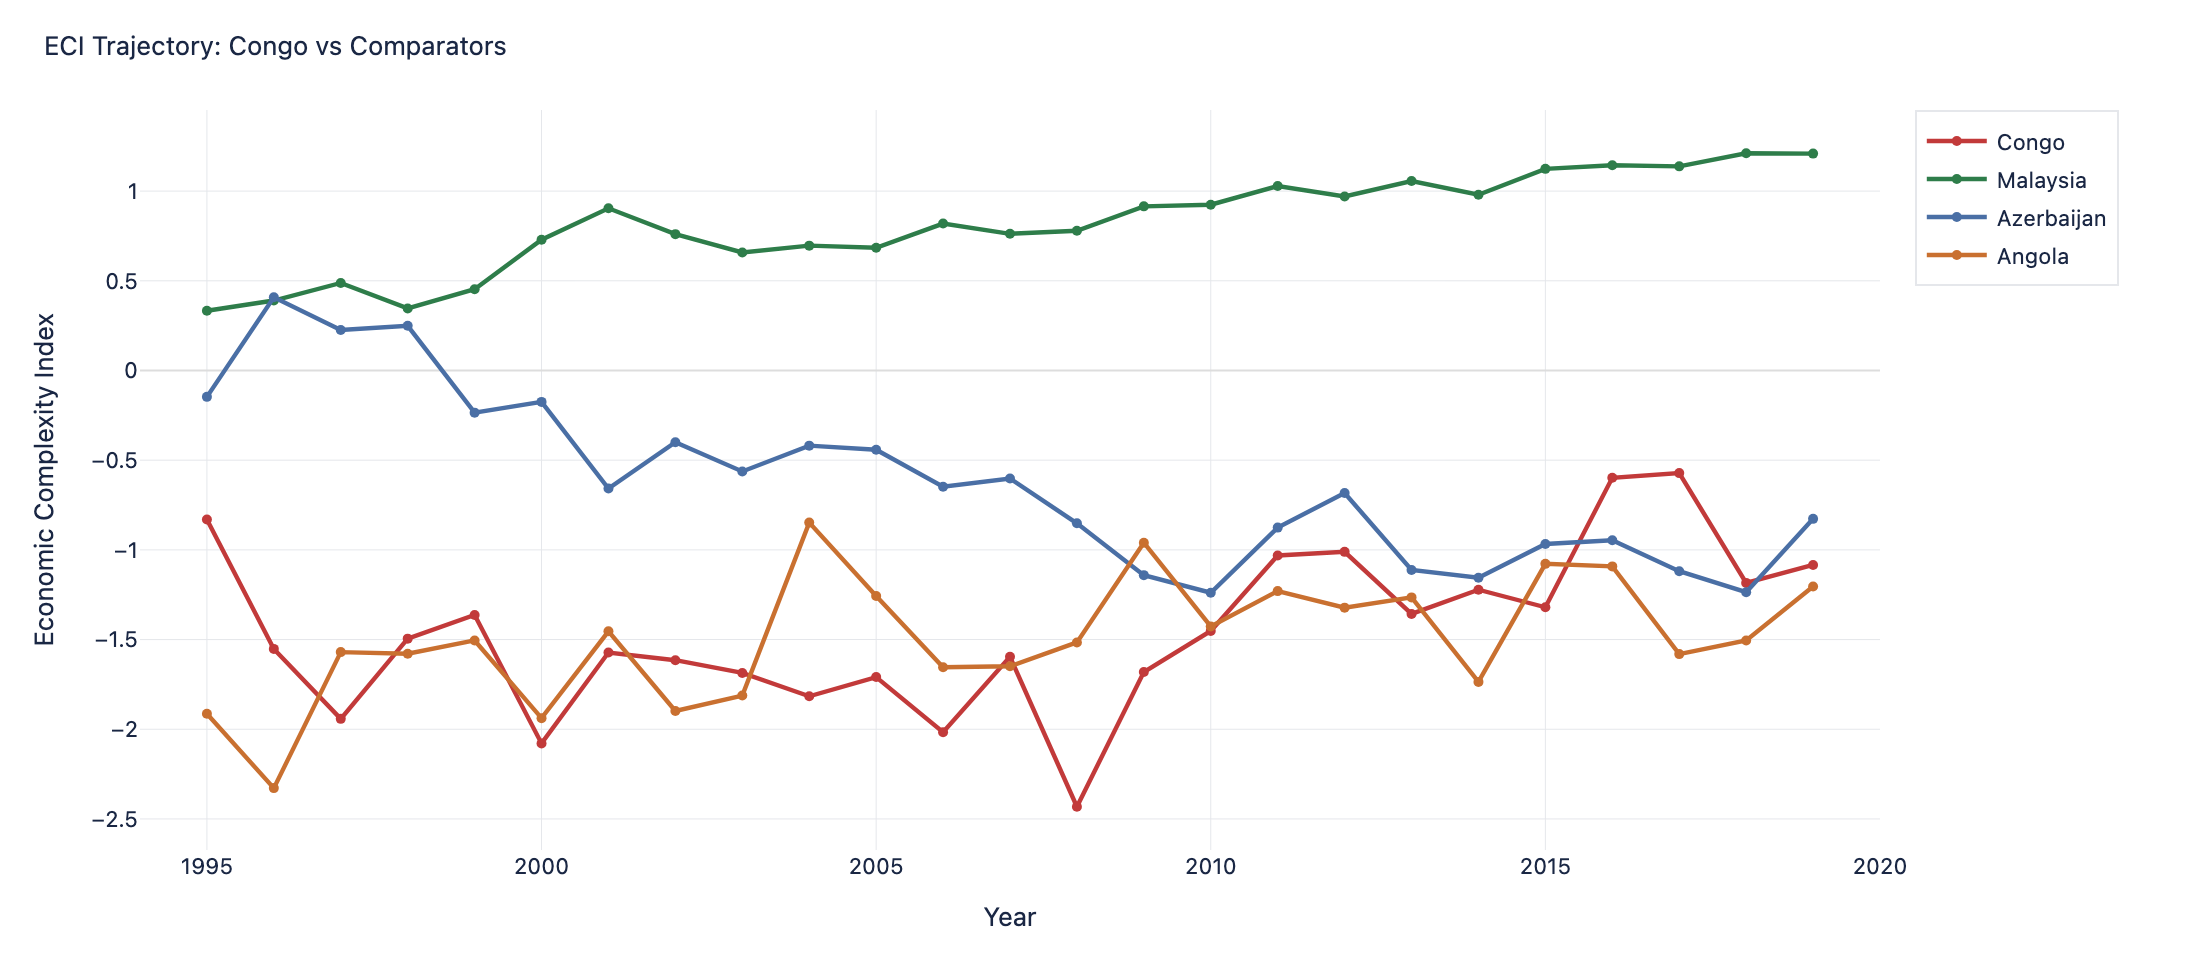
\includegraphics[width=0.95\textwidth]{descriptive/16_eci_traj_congo_comparators}
\caption{ECI trajectory: Republic of the Congo and comparators}
\label{fig:congo_comparators}
\end{figure}

\subsection{Policy Recommendations}

\paragraph{Strengthening human capital accumulation.} Improving human capital outcomes requires stabilizing and increasing investment in education and health, which has historically been volatile and closely tied to oil revenues. Given the ROC's low labour productivity, targeted investment in technical and vocational education in sectors such as agriculture, logistics, and construction could accelerate the reallocation of labour away from low-productivity informal activities.

\paragraph{Fiscal discipline and resource revenue management.} The ROC's fiscal position is highly procyclical. Adopting a credible fiscal rule anchored to a structural oil price benchmark would help delink expenditure from short-term commodity fluctuations.

\paragraph{Institutional quality and infrastructure systems.} Strengthening public financial management systems, enhancing transparency in the management of natural resource revenues, and reinforcing anti-corruption institutions remain central. The ROC's electricity sector represents a binding constraint, where despite significant hydroelectric potential, unreliable supply and limited grid coverage continue to raise production costs.


% ── Azerbaijan ──────────────────────────────────────────────
\section{Azerbaijan}

\subsection{Overview}

Azerbaijan is the largest and most populous country in the South Caucasus, classified as upper-middle-income, with around 10 million inhabitants. The oil and gas sectors dominate the country's economy, accounting for roughly 90\% of export revenues and 50\% of GDP (IEA, 2023; BP, 2024). Governance indicators are weak, with Azerbaijan scoring in the bottom quartile on V-Dem's political corruption index.

Fiscal management is anchored by the State Oil Fund of Azerbaijan (SOFAZ), a sovereign wealth fund established in 1999, though transfers to the state budget have at times exceeded the fund's own savings rules (IMF, 2023). The country holds a Ba1/BB+/BB+ sovereign credit rating.

\subsection{Why We Chose This Country}

Azerbaijan's economy remains heavily dependent on oil and gas. The country's ECI declined between 1995 and 2019, even as GDP growth averaged 6.59\% over the same period. Almost half of non-oil exports are themselves related to hydrocarbons, suggesting the country is even less diversified than aggregate statistics suggest.

Despite continued reliance on hydrocarbons, geopolitical developments have opened new markets for Azerbaijani gas. Following Russia's full-scale invasion of Ukraine in February 2022, European countries positioned Azerbaijan as a strategically attractive alternative supplier. Azerbaijan has increased its gas exports to Europe by 56\% since 2021 (Birbayeva, 2026).

\subsection{Economic Structure}

Azerbaijan's economy is primarily based on oil, with the rest of the sectors trailing behind. In 2024, non-oil sectors include trade and vehicle repair (10.7\% of GDP), transport and warehousing (7.0\%), construction (6.7\%), agriculture (5.7\%), tourism (2.4\%), and information and communications (1.9\%). From 2018 to 2023, Azerbaijan has advanced its ECI, however, the ECI remains relatively low in absolute terms, ranking 95th.

\paragraph{Fiscal and financial position.} Azerbaijan's financial system has improved since the 2015 crisis. The 2015--16 banking crisis led to widespread devaluations and recession. Since then, authorities have begun closing non-viable banks and addressing Non-Performing Loans. The aggregate NPL ratio fell from 21\% at end-2016 to 2.7\% by mid-2024.

The fiscal rule, introduced in 2018, set upper limits on oil revenue spending based on net financial assets (Azertac, 2018), though governance weaknesses persisted. The absence of binding authority within SOFAZ's Supervisory Board to reject presidential withdrawal orders also threatened fiscal sustainability (IMF, 2025).

\subsection{Human Capital}

Azerbaijan's Human Capital Index improved by 15\% between 1995 and 2019 (from 2.91 to 3.35), though it remains below regional peers (World Bank, 2022). The country is locked in a low-productivity, low-skill cycle. Weak non-oil labour demand suppresses returns to education; firms identify inadequate skills and low digital literacy as key constraints.

\subsection{Infrastructure and Dutch Disease}

Azerbaijan's infrastructural development since independence has been focused on energy export infrastructure (pipelines). However, other infrastructure sectors have declined. Infrastructure spending has been mainly concentrated on export pipelines and in the capital Baku. The railway sector shows a contrasting story, with rail goods transported dropping from 26.5 million tons in 2006 to 15.5 million tons in 2016 (Asian Development Bank, 2021).

The spending effect crowded out non-oil tradable sectors. Azerbaijan suffers from ``relative de-industrialization'' in the non-oil tradable sector, while the non-tradable sector substantially expanded during the 2000--2007 period (Hasanov, 2013).

\subsection{Governance and Institutions}

Azerbaijan's political stability index improved marginally between 1995 and 2019, while rule of law remained virtually unchanged, both below sample averages. The political system is characterised by autocratic presidentialism with neopatrimonial structures and extensive rent capture (Franke, 2009). Media is predominantly state-controlled and independent journalists face criminal charges.

\subsection{Peer Comparison}

Malaysia serves as a potential counterfactual. Both countries were upper-middle-income hydrocarbon economies in the mid-1990s with comparable ECI levels, yet Malaysia sustained a continuous upward trajectory to $+1.1$ by 2019 while Azerbaijan collapsed to $-1.2$ by the mid-2000s. Two binding constraints explain this underperformance: severely inadequate rule of law (consistently around $-0.7$ versus Malaysia's $+0.5$), and extreme hydrocarbon concentration that crowds out non-oil tradable activity through Dutch Disease channels.

\begin{figure}[H]
\centering
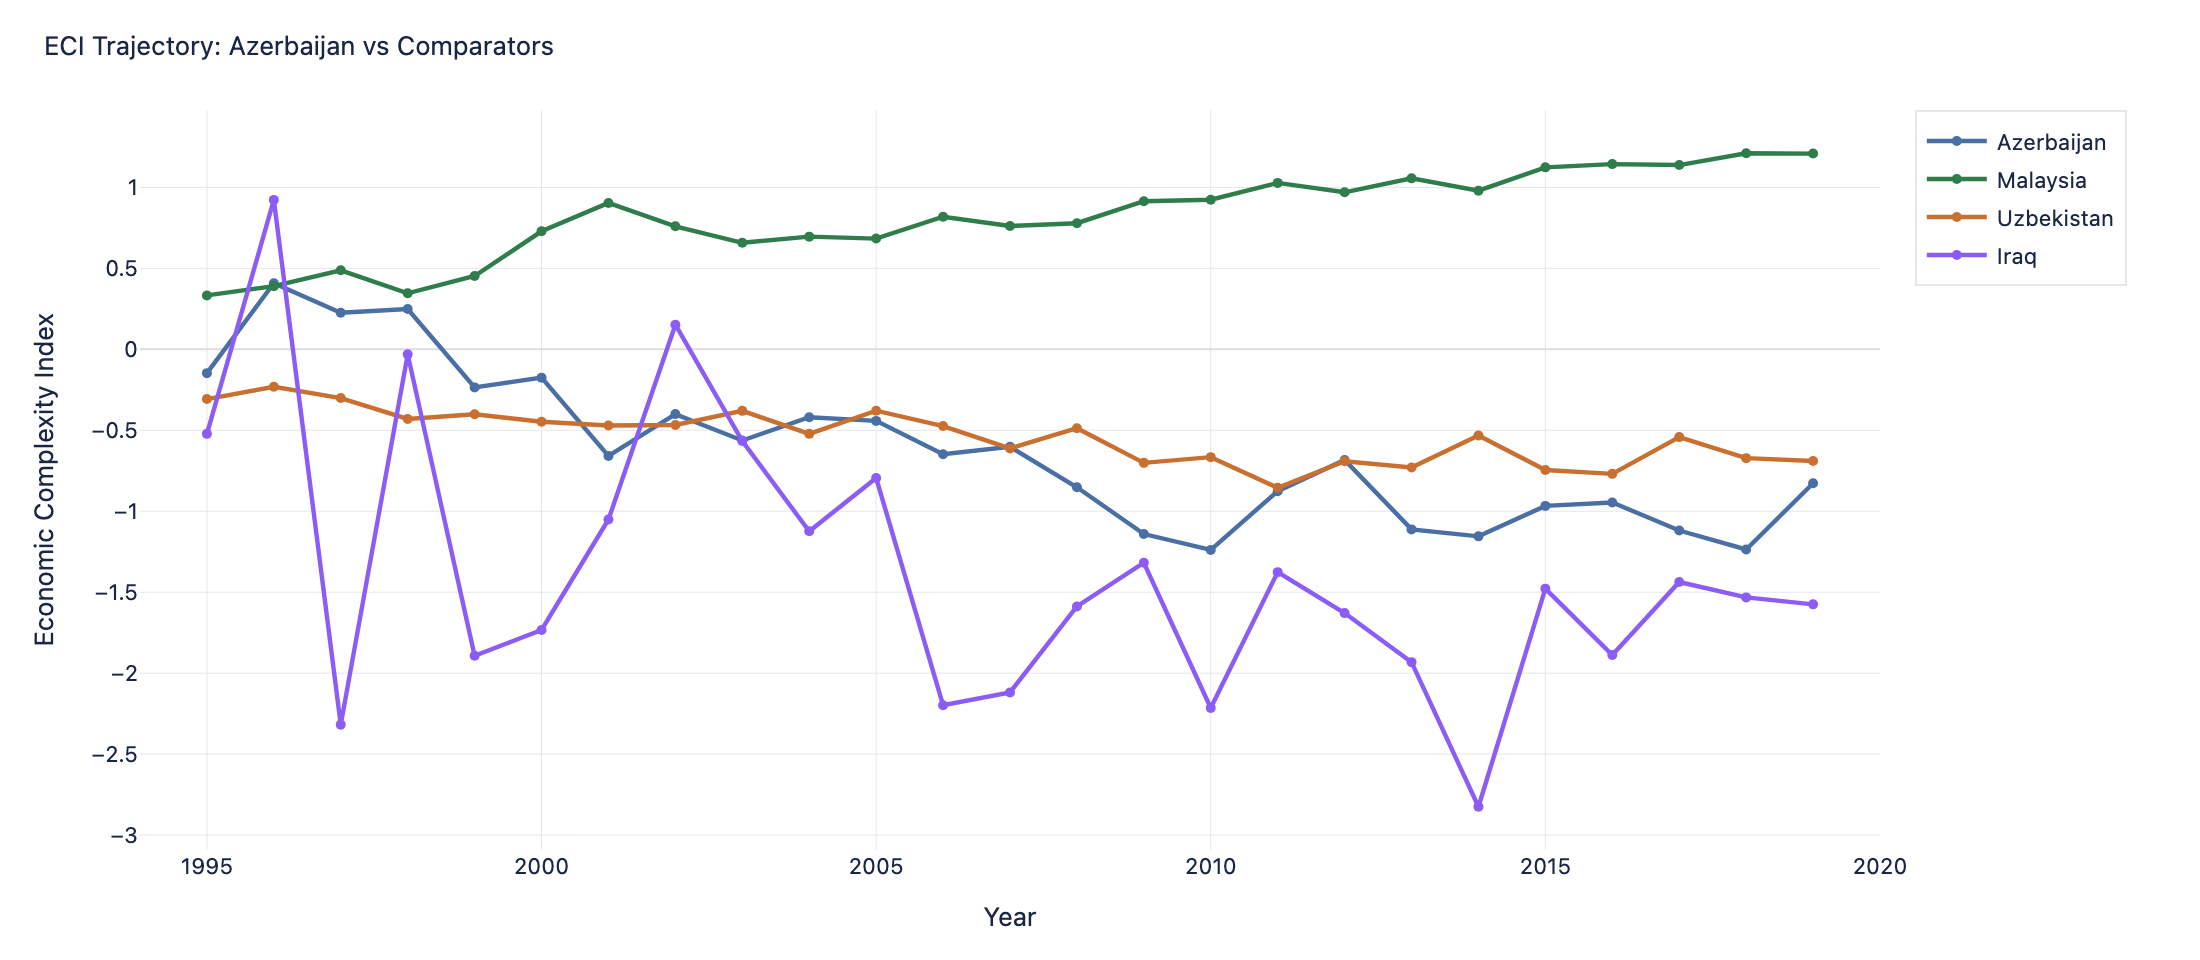
\includegraphics[width=0.95\textwidth]{descriptive/17_eci_traj_az_comparators}
\caption{ECI trajectory: Azerbaijan and comparators}
\label{fig:az_comparators}
\end{figure}

\subsection{Policy Recommendations}

\paragraph{Establish independent mechanisms to mitigate rent capture.} Rent capture by ruling government links directly suppresses private sector innovation. This calls for oversight bodies for sovereign wealth fund governance, transparency for large enterprises, competitive procurement in public contracting, and sufficient judicial independence.

\paragraph{Invest in human capital and productive diversification.} Azerbaijan should prioritise sectors closely related to its existing export basket: petrochemicals, agro-processing, logistics, and renewable energy engineering.

\paragraph{Create independent institutions for economic data production and transparency.} This requires an independent national statistics office with statutory protections and international methodological standards, alongside a fiscal council mandated to publish non-oil deficit projections and SOFAZ sustainability assessments.


% ── Chile ──────────────────────────────────────────────────
\section{Chile}

\subsection{Overview}

Chile sits along the western coast of South America, with a population of approximately 19.5 million. It is classified as high-income by the World Bank. Chile is the world's largest copper producer and second-largest lithium producer, with mining contributing roughly 12\% of GDP and 57\% of exports (ITA, 2025; USGS, 2024).

Fiscal governance is strong. A structural balance rule ties fiscal spending to long-run copper prices (Marcel, 2011), supported by two sovereign wealth funds (ESSF and PRF) and an independent inflation-targeting central bank, contributing to the highest sovereign credit rating in the region (A2/A/A-).

\subsection{Why We Chose This Country}

Chile satisfies some of the institutional prerequisites that the literature identified as potential binding constraints on diversification: democratic governance, solid fiscal position, and developed infrastructure. Despite this, its ECI has been declining since the mid-2000s, worker productivity sits 50\% below the OECD average, and income inequality remains among the highest in the OECD.

\subsection{Economic Structure and Trajectory}

Chile's commodity dependence stretches back to the nitrate boom following the War of the Pacific (1879--1883). Copper gradually replaced nitrates and became central to state revenues after CODELCO's creation in 1971. Post-1973 liberalisation and the democratic transition fuelled average growth of 6.5\% through the 1990s.

Chile built a layered fiscal framework to manage commodity revenues countercyclically. The structural balance rule (2001) formalised this, and the 2006 Fiscal Responsibility Law created the ESSF and PRF as dedicated savings vehicles.

Chile's ECI peaked at approximately $-0.05$ in the mid-2000s and has since declined to around $-0.30$ in 2022. Its export basket has become less diversified over time, with products clustered around copper, lithium, molybdenum, wood pulp, and fresh fruit in the ``periphery'' of the product space (Hidalgo et al., 2007).

\subsection{Human Capital}

Chile's human capital reveals a quantity-quality gap. Average schooling of approximately 10 years places the country among the most educated in Latin America, yet PISA mathematics scores sit 60 points below the OECD average (OECD, 2024). R\&D expenditure at 0.34\% of GDP is roughly one-sixth of the 2022 OECD average.

Worker output is approximately 50\% below the OECD average (OECD, 2022), as workers tend to be highly productive only in the mining sectors. Antofagasta, the country's main mining region, records labour productivity 120\% above Chile's national average (OECD, 2024b).

\subsection{Infrastructure and Technology}

Chile's physical infrastructure is adequate by Latin American standards but still has clear bottlenecks. Railroad infrastructure quality is ranked 70th out of 103 countries (WEF, 2019). The northern and southern rail systems operate on different gauges with no through connection.

Salinas (2021) estimates that closing Chile's infrastructure gap relative to comparable advanced economies could raise complex exports by roughly 23\%, indicating that transport infrastructure acts as a direct constraint.

\subsection{Governance and Institutions}

Chile ranks between the 84th and 91st global percentile across all six World Governance Indicators. Weaknesses persist at the operational level: contract enforcement is slow and costly by OECD standards (World Bank, 2020). The failed constitutional processes of 2022 and 2023 generated political instability.

\subsection{Natural Resource Industry and Supply Chain}

The mining sector comprises 363 producing facilities across 17 commodity groups, generating an estimated USD 62 billion in annual mineral value (2024). Copper accounts for \$48.3 billion of this total. Production is heavily concentrated in three northern regions of Antofagasta, Tarapac\'{a}, and Atacama.

Forward linkages are more limited. Chile exports primarily in concentrate and refined form. Approximately 54\% of copper exports go to China for downstream processing, while lithium carbonate is shipped to battery manufacturers in East Asia.

\begin{figure}[H]
\centering
\includegraphics[width=0.9\textwidth]{image21}
\caption{Production value by mineral category, estimated 2024 (USD)}
\label{fig:chile_treemap}
\end{figure}

\subsection{Peer Comparison}

\textbf{Zambia} is similarly copper-dependent but at roughly one-eighth of Chile's GDP per capita. The country defaulted on its Eurobond obligations in 2020. \textbf{Botswana} used diamond revenues to rise from extreme poverty to upper-middle-income status, maintaining fiscal surpluses, yet diamonds still account for roughly 80\% of merchandise exports and its ECI remains among the lowest in the world. Both Chile and Botswana save during booms and maintain fiscal discipline, but neither has truly solved the diversification problem. \textbf{Norway} represents an aspirational peer, with R\&D spending (2\% of GDP vs.\ 0.34\%) reflecting a fundamentally different investment model.

\subsection{Policy Recommendations}

\paragraph{Rebuild the Economic and Social Stabilisation Fund.} The ESSF fell from USD 20 billion (14\% of GDP) in 2008 to approximately USD 5 billion (1.5\%) by 2024. Rebuilding the fund to 5--8\% of GDP would protect investment programmes from the next commodity downturn.

\paragraph{Direct lithium revenues toward education quality and applied research.} Norway's petroleum sector illustrates the mechanism: research institutions such as SINTEF and the University of Stavanger were operating in oil-producing regions (Ryggvik, 2015). Earmarking a defined share of lithium rents for applied research institutes in the northern mining corridor would create similar knowledge spillovers.

\paragraph{Build the domestic mining supply chain through credit access and procurement policy.} The upstream services sector is the most realistic near-term diversification channel. Procurement preferences for domestic suppliers and dedicated CORFO credit lines with risk-sharing facilities can direct capital where diversification is most likely to originate.

\paragraph{Invest in logistics infrastructure along the northern mining corridor.} Port facilities at Antofagasta and Mejillones are approaching capacity limits. Investing in port expansion, rail standardisation, and energy connections along the northern corridor would do more for export competitiveness than any further tariff reduction.


% ══════════════════════════════════════════════════════════════
\chapter{Final Remarks}
% ══════════════════════════════════════════════════════════════

This study examines how emerging market economies have struggled to translate natural resource extraction into higher value-added industrial activity, and which economic, institutional, and policy conditions explain cross-country divergence. It follows two complementary approaches, econometrics and machine learning methods, and analyses three case studies.

\textbf{Industrial upgrading in resource-rich economies is fundamentally a question of structural transformation.} Three pillars emerge as the most robust determinants of economic complexity: domestic credit to the private sector (a proxy for financial depth), infrastructure capacity associated with access to electricity, and human capital.

\textbf{The three case studies contextualise these findings across different institutional and developmental settings.} The ROC represents a severe form of persistent underperformance, ranking amid the worst in ECI. Conversely, Azerbaijan presents a revealing case in which GDP grew but ECI declined, consistent with Dutch Disease. Chile offers a distinct configuration, in which strong institutions coexist with a declining ECI since the mid-2000s, where the binding constraint is human capital quality. Together, the three cases show that the constraints on industrial upgrading shift as institutional and economic conditions improve, and that no single policy lever is sufficient across all settings.

\textbf{The forward-looking projections to 2030 reinforce the interpretation.} Countries such as Ecuador and Mongolia, where financial depth, human capital, and institutional quality are relatively strong for their current ECI levels, are positioned for continued complexity gains. Conversely, hydrocarbon-dominant economies such as Saudi Arabia and Libya face projected declines unless structural reforms are implemented.

\textbf{The policy implications are consistent and mutually reinforcing across the quantitative and case study evidence.} Deepening financial systems and expanding access to credit for non-extractive sectors constitutes the most consistent policy lever. Investment in human capital must be counter-cyclical and structurally insulated from commodity price volatility. The evidence points toward a consistent policy implication: the most effective pathway for resource-rich developing economies is not to abandon reliance on natural resources but to systematically transform resource rents into the structural foundations needed to sustain long-term productive diversification: financial development, human capital, and reliable infrastructure.


% ══════════════════════════════════════════════════════════════
\chapter*{References}
\addcontentsline{toc}{chapter}{References}
% ══════════════════════════════════════════════════════════════

\begin{flushleft}
\setlength{\parskip}{4pt}

Acemoglu, D., Johnson, S. and Robinson, J.A. (2001) `The colonial origins of comparative development: an empirical investigation', \textit{American Economic Review}, 91(5), pp.~1369--1401.

Acemoglu, D., Johnson, S. and Robinson, J.A. (2003) `An African success story: Botswana', in Rodrik, D. (ed.) \textit{In Search of Prosperity}. Princeton University Press, pp.~80--119.

Acemoglu, D., Naidu, S., Restrepo, P. and Robinson, J.A. (2019) `Democracy does cause growth', \textit{Journal of Political Economy}, 127(1), pp.~47--100.

Aghion, P., Angeletos, G.-M., Banerjee, A. and Manova, K. (2010) `Volatility and growth: credit constraints and the composition of investment', \textit{Journal of Monetary Economics}, 57(3), pp.~246--265.

Alves, A.C. (2013) `Chinese economic statecraft: a comparative study of China's oil-backed loans in Angola and Brazil', \textit{Journal of Current Chinese Affairs}, 42(1), pp.~99--130.

Asian Development Bank (2021) \textit{Project Administration Manual: Republic of Azerbaijan: Railway Sector Development Program}. Manila: ADB.

AZERTAC (2018) `New fiscal rule signed into law', \textit{Azerbaijan State News Agency}, 24 August.

Belloni, A., Chernozhukov, V. and Hansen, C. (2014) `High-dimensional methods and inference on structural and treatment effects', \textit{Journal of Economic Perspectives}, 28(2), pp.~29--50.

Bhattacharyya, S. and Collier, P. (2014) `Public capital in resource rich economies: is there a curse?', \textit{Oxford Economic Papers}, 66(1), pp.~1--24.

Birbayeva, A. (2026) `Azerbaijan boosts gas exports to Europe by 56\%', \textit{The Astana Times}, 4 March.

Boschini, A.D., Pettersson, J. and Roine, J. (2007) `Resource curse or not: a question of appropriability', \textit{Scandinavian Journal of Economics}, 109(3), pp.~593--617.

BP (2024) \textit{BP Statistical Review of World Energy}. London: BP.

Breiman, L. (2001) `Random forests', \textit{Machine Learning}, 45(1), pp.~5--32.

Broken Chalk (2020) `Educational challenges in Congo'.

Collier, P. and Hoeffler, A. (2004) `Greed and grievance in civil war', \textit{Oxford Economic Papers}, 56(4), pp.~563--595.

Corden, W.M. and Neary, J.P. (1982) `Booming sector and de-industrialisation in a small open economy', \textit{Economic Journal}, 92(368), pp.~825--848.

FAO and EFI (2018) \textit{Making forest concessions in the tropics work to achieve the 2030 Agenda}. FAO Forestry Paper No. 180. Rome: FAO.

Franke, A., Gawrich, A. and Alakbarov, G. (2009) `Kazakhstan and Azerbaijan as post-Soviet rentier states', \textit{Europe-Asia Studies}, 61(1), pp.~109--140.

Freedom House (2024) \textit{Nations in Transit 2024: Azerbaijan Country Report}. Washington, DC.

Gylfason, T. (2001) `Natural resources, education, and economic development', \textit{European Economic Review}, 45(4--6), pp.~847--859.

Hair, J.F., Black, W.C., Babin, B.J. and Anderson, R.E. (2019) \textit{Multivariate Data Analysis}. 8th edn. Cengage.

Hasanov, F. (2013) `Dutch disease and the Azerbaijan economy', \textit{Communist and Post-Communist Studies}, 46(4), pp.~463--480.

Hausmann, R., Hwang, J. and Rodrik, D. (2007) `What you export matters', \textit{Journal of Economic Growth}, 12(1), pp.~1--25.

Hausmann, R., Rodrik, D. and Velasco, A. (2005) \textit{Growth diagnostics}. Growth Lab Working Paper. Harvard University.

Havr\'{a}nek, T., Horv\'{a}th, R. and Zeynalov, A. (2016) `Natural resources and economic growth: a meta-analysis', \textit{World Development}, 88, pp.~134--151.

Hidalgo, C.A. and Hausmann, R. (2009) `The building blocks of economic complexity', \textit{Proceedings of the National Academy of Sciences}, 106(26), pp.~10570--10575.

Hidalgo, C.A., Klinger, B., Barab\'{a}si, A.-L. and Hausmann, R. (2007) `The product space conditions the development of nations', \textit{Science}, 317(5837), pp.~482--487.

Hoerl, A.E. and Kennard, R.W. (1970) `Ridge regression: biased estimation for nonorthogonal problems', \textit{Technometrics}, 12(1), pp.~55--67.

IEA (2023) \textit{Azerbaijan Energy Profile}. Paris: IEA.

IMF (2016) \textit{Republic of Azerbaijan: 2016 Article IV Consultation}. IMF Country Report No. 16/296.

IMF (2023) \textit{Azerbaijan: Article IV Consultation Staff Report}. Washington, DC.

IMF (2024a) \textit{Republic of Congo: Selected Issues}. IMF Country Report No. 24/252.

IMF (2025a) \textit{World Economic Outlook Database}. Washington, DC.

IMF (2025b) \textit{Republic of Azerbaijan: 2025 Article IV Consultation}. IMF Country Report No. 25/98.

IMF (2025e) \textit{Chile: 2024 Article IV Consultation Staff Report}. IMF Country Report No. 25/37.

IMF (2026) `IMF staff completes 2026 Article IV mission to Azerbaijan', \textit{IMF Press Release}, 19 February.

Isham, J., Woolcock, M., Pritchett, L. and Busby, G. (2005) `The varieties of resource experience', \textit{World Bank Economic Review}, 19(2), pp.~141--174.

ITA (2025) `Chile -- Mining', \textit{Country Commercial Guide}. U.S. Department of Commerce.

Jolliffe, I.T. (2002) \textit{Principal Component Analysis}. 2nd edn. Springer.

Kutner, M.H., Nachtsheim, C.J., Neter, J. and Li, W. (2004) \textit{Applied Linear Statistical Models}. 5th edn. McGraw-Hill.

Lashitew, A.A., Ross, M.L. and Werker, E. (2020) `What drives successful economic diversification in resource-rich countries?', \textit{World Bank Research Observer}, 36(2), pp.~164--196.

Lederman, D. and Maloney, W.F. (2007) \textit{Natural Resources: Neither Curse nor Destiny}. Stanford University Press.

MacQueen, J. (1967) `Some methods for classification and analysis of multivariate observations', in \textit{Proceedings of the Fifth Berkeley Symposium}, Vol. 1, pp.~281--297.

Manzano, O. and Rigobon, R. (2001) \textit{Resource curse or debt overhang?} NBER Working Paper No. 8390.

Marcel, M. (2011) `The structural balance rule in Chile: ten years, ten lessons', IDB Discussion Paper No. IDB-DP-184.

Mehlum, H., Moene, K. and Torvik, R. (2006) `Institutions and the resource curse', \textit{Economic Journal}, 116(508), pp.~1--20.

Mlachila, M. and Ouedraogo, R. (2020) `Financial development curse in resource-rich countries', \textit{Quarterly Review of Economics and Finance}, 76, pp.~84--96.

OECD (2017) \textit{Making Decentralisation Work in Chile}. OECD Publishing.

OECD (2022) \textit{OECD Economic Surveys: Chile 2022}. Paris: OECD Publishing.

OECD (2024a) \textit{Education at a Glance 2024}. Paris: OECD Publishing.

OECD (2025) \textit{OECD Economic Surveys: Chile 2025}. Paris: OECD Publishing.

Piketty, M.-G., Singer, B. and Karsenty, A. (2008) `Regulating industrial forest concessions in Central Africa and South America', \textit{Forest Ecology and Management}, 256(7), pp.~1498--1508.

Poelhekke, S. and van der Ploeg, F. (2010) \textit{Do natural resources attract FDI?} DNB Working Paper No. 266.

Ross, M.L. (2015) `What have we learned about the resource curse?', \textit{Annual Review of Political Science}, 18, pp.~239--259.

Ryggvik, H. (2015) `A short history of the Norwegian oil industry', \textit{Business History Review}, 89(1), pp.~3--41.

Sachs, J.D. and Warner, A.M. (1995) \textit{Natural resource abundance and economic growth}. NBER Working Paper No. 5398.

Sachs, J.D. and Warner, A.M. (2001) `The curse of natural resources', \textit{European Economic Review}, 45(4--6), pp.~827--838.

Salinas, G. (2021) `Chile: a role model of export diversification policies?', IMF Working Paper WP/21/148.

S{\o}reide, T. (2007) \textit{Forest concessions and corruption}. U4 Issue 2007:3. Bergen: CMI.

Tibshirani, R. (1996) `Regression shrinkage and selection via the lasso', \textit{Journal of the Royal Statistical Society, Series B}, 58(1), pp.~267--288.

Transparency International (2025) `CPI 2024 for Eastern Europe and Central Asia', 11 February.

USGS (2024) \textit{Mineral Commodity Summaries 2024}. Reston, VA.

Van der Ploeg, F. and Poelhekke, S. (2009) `Volatility and the natural resource curse', \textit{Oxford Economic Papers}, 61(4), pp.~727--760.

Van der Ploeg, F. and Venables, A.J. (2011) `Harnessing windfall revenues', \textit{Economic Journal}, 121(551), pp.~1--30.

Venables, A.J. (2016) `Using natural resources for development: why has it proven so difficult?', \textit{Journal of Economic Perspectives}, 30(1), pp.~161--184.

World Bank (2020) \textit{Doing Business 2020}. Washington, DC.

World Bank (2022a) \textit{Azerbaijan Human Capital Review}. Washington, DC.

World Bank (2023a) \textit{Republic of Congo: Country Economic Memorandum}. Washington, DC.

World Bank (2023b) \textit{Republic of Congo Economic Update: Reforming Fossil Fuel Subsidies}. Washington, DC.

World Bank (2025) \textit{Republic of Congo Economic Update}. 12th edn. Washington, DC.

World Bank (2026) \textit{World Development Indicators}. Washington, DC.

Zou, H. and Hastie, T. (2005) `Regularization and variable selection via the elastic net', \textit{Journal of the Royal Statistical Society, Series B}, 67(2), pp.~301--320.

\end{flushleft}


% ══════════════════════════════════════════════════════════════
\begin{appendices}
% ══════════════════════════════════════════════════════════════

\chapter{Data Sources}

\section{Economic Complexity Index}

ECI is constructed from goods trade data at the HS4 level of product classification. Countries and products are arranged into a binary matrix indicating whether a country holds a revealed comparative advantage in each product, defined as a share of that product in the country's exports exceeding its share in world exports. From this matrix, two quantities are derived: the diversity of each country's export basket and the ubiquity of each product it exports. These are then refined iteratively to account not only for how many products a country exports competitively, but for how rare those products are across other exporters. The resulting index summarises an economy's productive sophistication and serves as the proxy for value chain upgrading capacity throughout this analysis.

Employing ECI as an outcome carries limitations. Because it is derived from trade data, it excludes value-added activity that is domestically consumed, likely understating the degree of productive upgrading. It also omits the services sector. Finally, ECI measures accumulated productive know-how rather than the dollar value generated by value-added industries. Despite these limitations, ECI aligns well with the analytical framework of this study and offers wide availability across countries and years, covering the full panel from 1995 to 2019 with minimal gaps.

\section{World Bank Data}

The World Development Indicators (WDI) database provides a comprehensive set of statistics tracking economic, social, and environmental performance across countries worldwide (World Bank, 2026). We draw 26 WDI variables covering natural resource rents, the sectoral composition of GDP, savings and resource depletion indicators, employment shares, infrastructure proxies, financial indicators, demographics, and trade openness.

\section{IMF WEO}

We supplement the World Bank data with macroeconomic indicators from the IMF's World Economic Outlook: GDP per capita at constant prices in purchasing power parity, general government revenue as a share of GDP, general government net debt as a share of GDP, and the general government structural fiscal balance as a share of potential GDP (IMF, 2025).

\section{IMF Investment and Capital Stock Dataset}

We extract gross fixed capital formation (GFCF) as a share of GDP at constant prices and general government primary net lending as a share of GDP. These complement the WEO fiscal indicators by capturing the investment dimension of macroeconomic policy.

\section{V-Democracy}

We include indicators from the Varieties of Democracy (V-Dem) dataset, which provides expert-coded measures of political institutions, governance, and democracy. These indicators allow us to account for the role of governance and institutional capacity in the relationship between natural resources and value chain upgrading.

\section{Penn World Table}

We draw on data from the Penn World Table version 11.0 (PWT 11.0), specifically human capital variables, the capital depreciation rate and capital stock of countries (Feenstra, Inklaar, and Timmer, 2015).

\section{CEPII}

We include a binary indicator identifying whether a country is landlocked, sourced from the GeoDist database maintained by CEPII (Mayer and Zignago, 2011).

\section{Natural Resources Stock and Production}

We complement the rent-based proxies from the World Bank with direct measures of natural resource production quantities, reserves, and prices from the Energy Institute's Statistical Review of World Energy, Our World in Data, and the USGS Data Series 140 (Kelly and Matos, 2014).


\chapter{Processing Data}

\section{Countries Excluded Due to Data Availability}

\begin{table}[H]
\centering
\caption{Countries excluded from the sample}
\small
\begin{tabular}{@{}llp{10cm}@{}}
\toprule
\textbf{Country} & \textbf{Code} & \textbf{Reason} \\
\midrule
French Guiana & GUF & Little economic data; minor gold producer \\
North Korea & PRK & Extensive missing economic data; reliability concerns \\
Taiwan & TWN & Limited natural resources, poor data coverage \\
New Caledonia & NCL & French territory; governance structure complicates analysis \\
South Sudan & SSD & Extensive missing economic data \\
Cuba & CUB & Extensive missing economic data \\
Eritrea & ERI & Poor economic data coverage \\
Timor-Leste & TLS & Highly local economy; poor economic data \\
Afghanistan & AFG & Key variables missing \\
Turkmenistan & TKM & Key economic variables missing completely \\
Syria & SYR & Insufficient variables with decent coverage \\
Montenegro & MNE & ECI and human capital variables missing \\
Cambodia & KHM & Only features for 1 year; minor gold production \\
\bottomrule
\end{tabular}
\label{tab:excluded_countries}
\end{table}

\section{Imputation}

Linear interpolation estimates missing values between two observed data points by assuming a linear relationship. If a variable is observed at time $t_0$ with value $y_0$ and at time $t_1$ with value $y_1$, the interpolated value at time $t$ is:

\begin{equation}
y_t = y_0 + \frac{(y_1 - y_0)}{(t_1 - t_0)} \times (t - t_0)
\end{equation}

Extrapolation extends the same logic beyond observed values, capped at three years. Gaps exceeding this window are left for the KNN pass.

\section{K-Nearest Neighbours Imputation}

Where a country has no observed value for a given variable across the entire sample period, interpolation cannot proceed. These cells are filled using KNN imputation ($k=5$, distance-weighted). The median prediction error across all variables is 5.24\%. Performance is weaker for volatile time-series: inflation (31.1\%), real interest rates (36.4\%), and mineral rents (44.4\%).


\chapter{Clustering Techniques}

\section{Principal Component Analysis}

PCA transforms a set of potentially correlated variables into a smaller set of uncorrelated principal components. Given a data matrix $\mathbf{X}$ of dimension $n \times p$, PCA proceeds as follows:

\paragraph{Step 1: Standardization.}
$Z_{ij} = \frac{X_{ij} - \mu_j}{\sigma_j}$

\paragraph{Step 2: Covariance Matrix.}
$\Sigma = \frac{1}{n-1} Z^T Z$

\paragraph{Step 3: Eigendecomposition.}
$\Sigma \mathbf{v}_k = \lambda_k \mathbf{v}_k$

\paragraph{Step 4: Principal Component Scores.}
$PC = Z V$

The first two principal components together account for 69.5\% of total variance. PC1 explains 51.8\% and is driven by oil and natural gas; PC2 explains 17.7\% and captures mining activity.

\begin{figure}[H]
\centering

\includegraphics[width=0.95\textwidth]{descriptive/26_pca_loadings_heatmap}
\caption{PCA loadings heatmap: resource production profiles}
\label{fig:pca_loadings}
\end{figure}

\section{K-means Clustering Algorithm}

K-means minimises the within-cluster sum of squares:

\begin{equation}
WCSS = \sum_{j=1}^{k} \sum_{i \in C_j} \| x_i - \mu_j \|^2
\end{equation}

\section{Cluster Robustness}

\subsection{Choice of $k$}

\begin{figure}[H]
\centering
\includegraphics[width=0.9\textwidth]{image23}
\caption{Silhouette score across clusters}
\label{fig:silhouette}
\end{figure}

\subsection{Alternative Cluster Specifications}

\begin{figure}[H]
\centering

\includegraphics[width=0.9\textwidth]{cluster_robustness/silhouette_k3__1995}
\caption{Cluster map with $k=3$}
\end{figure}

\begin{figure}[H]
\centering

\includegraphics[width=0.9\textwidth]{cluster_robustness/silhouette_k4__1995}
\caption{Cluster map with $k=4$}
\end{figure}

\begin{figure}[H]
\centering

\includegraphics[width=0.9\textwidth]{cluster_robustness/silhouette_k6__1995}
\caption{Cluster map with $k=6$}
\end{figure}

\subsection{Alternative Specifications}

Three robustness checks vary one feature of the baseline pipeline at a time. Agreement is measured by the Adjusted Rand Index (ARI).

\begin{figure}[H]
\centering

\includegraphics[width=0.9\textwidth]{cluster_robustness/rob_A__1995_minerals_merged_k5}
\caption{Robustness A: Merged mineral commodities}
\end{figure}

\begin{figure}[H]
\centering

\includegraphics[width=0.9\textwidth]{cluster_robustness/rob_B__1995_pca3_k5}
\caption{Robustness B: Three principal components}
\end{figure}

\begin{figure}[H]
\centering

\includegraphics[width=0.9\textwidth]{cluster_robustness/rob_C__2019_standard_k5}
\caption{Robustness C: 2019-level production}
\end{figure}

\begin{figure}[H]
\centering

\includegraphics[width=0.9\textwidth]{cluster_robustness/stability_heatmap}
\caption{Cluster assignment stability across specifications}
\end{figure}

\begin{figure}[H]
\centering

\includegraphics[width=0.9\textwidth]{cluster_robustness/stability_world_map}
\caption{Country-level cluster stability map}
\end{figure}


\chapter{Regression Approach}

\section{Change in ECI as Dependent Variable}

Given the high persistence of ECI, we ran a regression with the change in ECI as the dependent variable as an additional robustness check. The results are robust to this specification.

\begin{figure}[H]
\centering
\adjustbox{max width=\linewidth}{\includegraphics{image32}}
\caption{Regression results: change in ECI as dependent variable}
\label{fig:change_eci}
\end{figure}

\section{Variance Inflation Factor (VIF)}

The VIF for variable $j$ is defined as:
\begin{equation}
VIF_j = \frac{1}{1 - R_j^2}
\end{equation}
where $R_j^2$ is the R-squared obtained from regressing variable $j$ on all remaining predictors. All variables fall below the conventional threshold of 5.

\begin{figure}[H]
\centering
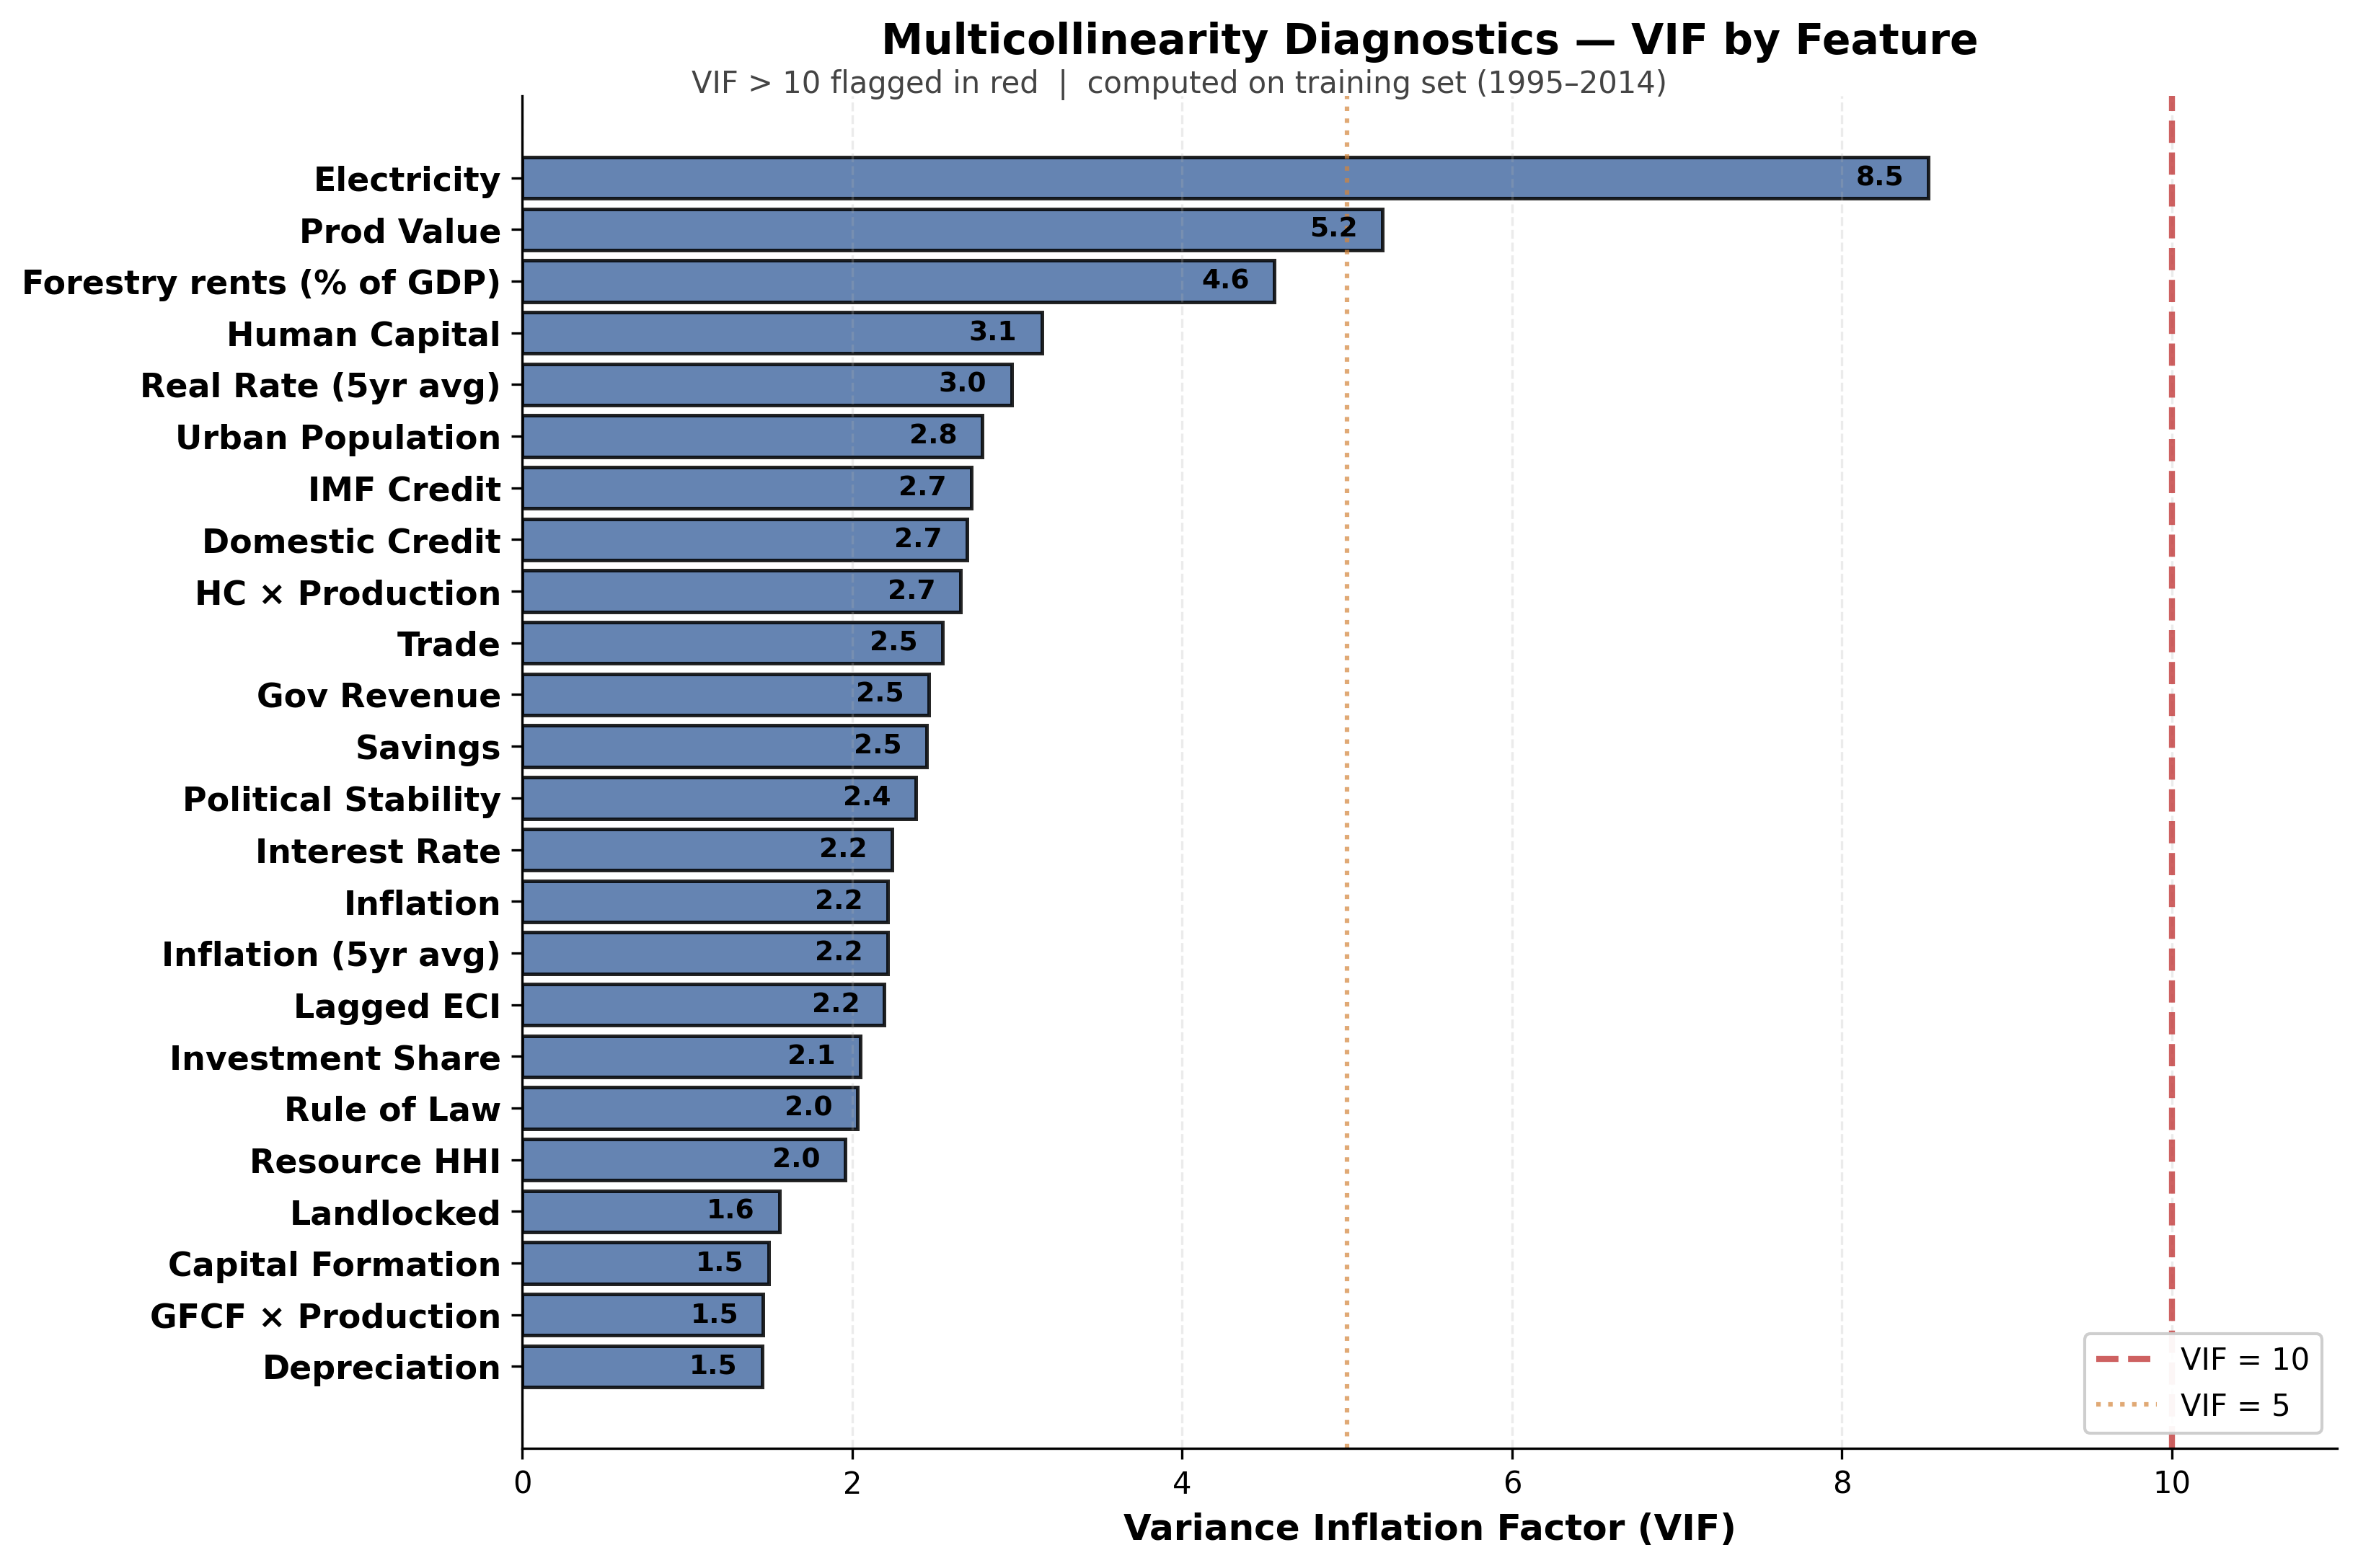
\includegraphics[width=0.9\textwidth]{appendix/vif_by_feature}
\caption{Multicollinearity diagnostics: VIF by feature}
\label{fig:vif}
\end{figure}


\chapter{Modelling Details}

\section{Regularization Techniques}

\subsection{LASSO Regression}

LASSO adds an L1 penalty to the least squares objective:
\begin{equation}
\min_{\beta} \left\{ \frac{1}{2n} \sum_{i=1}^{n} (y_i - x_i^T \beta)^2 + \lambda \sum_{j=1}^{p} |\beta_j| \right\}
\end{equation}

\subsection{Ridge Regression}

Ridge regression adds an L2 penalty:
\begin{equation}
\min_{\beta} \left\{ \frac{1}{2n} \sum_{i=1}^{n} (y_i - x_i^T \beta)^2 + \lambda \sum_{j=1}^{p} \beta_j^2 \right\}
\end{equation}

\subsection{Elastic Net}

Elastic Net combines L1 and L2 penalties:
\begin{equation}
\min_{\beta} \left\{ \frac{1}{2n} \sum_{i=1}^{n} (y_i - x_i^T \beta)^2 + \lambda \left( \alpha \sum_{j=1}^{p} |\beta_j| + \frac{1 - \alpha}{2} \sum_{j=1}^{p} \beta_j^2 \right) \right\}
\end{equation}

\subsection{Random Forest}

Random Forest is a non-parametric ensemble learning method (Breiman, 2001) that constructs a large number of decision trees on bootstrap samples, aggregating their predictions by averaging. We set $B = 500$ trees and tune $m$ via cross-validation. Variable importance is assessed through Mean Decrease in Impurity (MDI) and permutation importance (MDA).


\chapter{Model Extensions}

\section{Bootstrap Model Coefficients}

To test how sensitive the results are to the composition of countries in the sample, we run a country-level block bootstrap with 200 iterations. The main OLS findings survive resampling, with Human Capital and Rule of Law showing 100\% sign stability and their 95\% bootstrap confidence intervals excluding zero.

\begin{figure}[H]
\centering

\includegraphics[width=0.9\textwidth]{appendix/fig_A1_boot_reg_coefs}
\caption{OLS Regression: bootstrap coefficient confidence intervals}
\end{figure}

\begin{figure}[H]
\centering

\includegraphics[width=0.9\textwidth]{appendix/fig_A2_boot_ml_r2}
\caption{ML Models: test $R^2$ distribution}
\end{figure}

\begin{figure}[H]
\centering

\includegraphics[width=0.85\textwidth]{appendix/fig_A4b_boot_ml_coefs}
\caption{ML Models: bootstrap coefficient stability}
\end{figure}

\begin{figure}[H]
\centering

\includegraphics[width=0.85\textwidth]{appendix/fig_A3_boot_rf_importance}
\caption{Random Forest: bootstrap feature importance}
\end{figure}

\section{Leave-One-Country-Out (LOCO) Analysis}

For each of the 54 countries, we exclude all of its observations and refit both OLS specifications and all four ML models on the remaining 53 countries. Neither the OLS nor the ML findings are contingent on any single country's presence in the sample.

\begin{figure}[H]
\centering

\includegraphics[width=0.9\textwidth]{appendix/fig_A5_loco_ml_coef}
\caption{LOCO coefficient stability: ML models}
\end{figure}

\begin{figure}[H]
\centering

\includegraphics[width=0.9\textwidth]{appendix/fig_A6_loco_ml_r2}
\caption{LOCO $R^2$ stability: ML models}
\end{figure}

\begin{figure}[H]
\centering

\includegraphics[width=0.9\textwidth]{appendix/fig_A7_loco_reg_coef}
\caption{LOCO coefficient stability: OLS models}
\end{figure}

\begin{figure}[H]
\centering

\includegraphics[width=0.9\textwidth]{appendix/fig_A8_loco_reg_r2}
\caption{LOCO $R^2$ stability: OLS models}
\end{figure}


\end{appendices}

% ══════════════════════════════════════════════════════════════
% Terms of Reference (unnumbered)
% ══════════════════════════════════════════════════════════════
\clearpage
\chapter*{Terms of Reference}
\addcontentsline{toc}{chapter}{Terms of Reference}

{\large \textbf{Industrial Upgrading in Emerging Markets with Rich Natural Resources}}

\section*{Background}

Understanding the drivers of economic growth is central to development research and sovereign risk assessment. Countries with high-value-added industries tend to achieve stronger long-term growth, fiscal stability, and economic resilience. While natural resource wealth offers emerging markets opportunities for industrial upgrading, outcomes vary dramatically. This divergence is closely linked to sovereign creditworthiness.

\section*{Research Questions}

The project will identify economic indicators, institutional factors, and policy conditions that support or hinder industrial upgrading in resource-rich emerging markets.

\subsection*{Primary Questions}

How successful have emerging market economies been at developing value-added industries from natural resource extraction? What factors explain the divergence across countries?

\subsection*{Secondary Questions}

\begin{enumerate}
\item How sustainable are these shifts in terms of fiscal revenues, employment and export diversification?
\item How have they supported or hindered credit quality?
\item What policy levers and institutional conditions support or hinder the transition?
\end{enumerate}

\section*{Project Objectives}

\subsection*{Main Objective}

To develop a framework that identifies and analyses the economic and institutional drivers of industrial upgrading in resource-rich emerging markets, understanding how this is linked with credit risk.

\subsection*{Specific Objectives}

\begin{itemize}
\item Identify cross-country patterns to evaluate the predictors of industrial upgrading using supervised and unsupervised machine learning techniques.
\item Build econometric models, founded on economic theory and literature, to complement and validate machine learning approaches.
\item Conduct comparative country case studies to build a deeper understanding of local factors that influence industrial upgrading.
\item Generate actionable recommendations for sovereign risk assessments.
\item Deliver an Insights Report and a Presentation suitable for publication.
\end{itemize}

\section*{Scope}

This project focuses on emerging and developing economies, recognising their unique structural challenges and opportunities in resource-based development pathways. Rather than examining industrial growth broadly, the analysis specifically targets value-added industrial upgrading, the critical transition from raw material extraction to higher-value manufacturing and processing activities.

\section*{Research Methodology}

\subsection*{Literature Review}

The project draws on economic complexity and value-added upgrading (Hidalgo \& Hausmann, 2009) combined with the Growth Diagnostics Framework (Hausmann, Rodrik \& Velasco, 2005); Acemoglu \& Robinson's (2012) institutional economics framework; and Global Value Chain literature.

\subsection*{Analytical Approach}

\begin{itemize}
\item Unsupervised learning (PCA, Clustering) to identify country groupings.
\item Supervised learning (Ridge, Elastic Net, LASSO, Random Forest) to identify predictors.
\item Econometric panel data modelling to complement findings.
\item Paired case studies to examine mechanisms, governance factors, and policy interventions.
\end{itemize}

\section*{Project Phases and Timeline}

\subsection*{Phase 1: Exploratory Analysis (Oct--Dec 2025)}

Kick-off meeting, literature review, data cleaning, cluster analysis. Deliverables: ToR and progress presentation.

\subsection*{Phase 2: Supervised Modelling and Econometrics (Dec 2025 -- Jan 2026)}

Build and test supervised ML models, identify key predictors, select countries for case studies, econometric analysis.

\subsection*{Phase 3: Case Studies and Synthesis (Feb--Mar 2026)}

Conduct case studies, integrate quantitative and qualitative insights, draft final report. Final presentation to Moody's (late March 2026).

\subsection*{Final Deliverables}

Comprehensive research report, Moody's Insights report, presentation slides.

\end{document}
